\chapter[Our Framework at Work on the iTrust SWaT System]{Our Framework at Work: Reverse Engineering of the iTrust SWaT System}
\label{application}
%\linenumbers

\lettrine{I}{n} this chapter, our main objective is to apply the framework and methodology introduced in Chapter \ref{chap:proposal} to the case study of the iTrust SWaT system, as illustrated in Chapter \ref{casestudy}. The purpose of this analysis is to assess the effectiveness and potential of the proposed framework within the context of a system that closely replicates a real-world water treatment plant, albeit on a smaller scale.

\bigskip
Due to the complexity of the system and the limited space available in this thesis, we will not conduct a comprehensive analysis and reverse engineering of the entire system. Instead, \textbf{we will focus on specific parts} for analysis. We leave it to the reader or those interested in utilizing the proposed methodology and framework to complete the analysis, should they choose to do so.

By focusing on selective components and leaving room for further exploration, we strike a balance between providing valuable insights and acknowledging the potential for additional research. This approach empowers the reader and interested individuals to explore the iTrust SWaT system further and leverage the proposed methodology and framework for a more comprehensive analysis.
\vfill

\section{Preliminary Operations}
\label{sec:6_preliminar_operations}
Prior to beginning the actual analysis, several preliminary manual operations need to be conducted on the physical process dataset utilized as a case study, specifically the SWaT system dataset for the year 2015 as outlined in Section \ref{subsec:5_2015_datasets}. To simulate the data-capture process performed by Ceccato et al. using their scanning tool, the original dataset in XLSX format (proprietary to Microsoft Excel) was divided into multiple datasets in CSV format. Each of these datasets corresponds to the individual stages of the SWaT system and contains the respective registers. These resulting files were then saved in the directory specified by the \texttt{raw\_dataset\_directory} directive in the framework configuration file, \textit{config.ini}, ready to be used in the pre-processing phase.
Furthermore, the headers were manually renamed by adding a prefix from \texttt{P1\_} to \texttt{P6\_} to each register's name. This prefix indicates the stages, ensuring that each register is easily identifiable and linked to its corresponding stage.

\section{Planning the Analysis Strategy}
\label{sec:6_analysis_strategy}
The complexity of the system being analyzed necessitates the adoption of a deliberate strategy for the analysis. It is not feasible to rely on trial and error or attempt every possible combination between stages. The former approach may overlook crucial relationships between PLCs or between registers, while the latter may result in excessive and unproductive efforts if the specific portion of the system being analyzed lacks significant information or relationships. 
A sound analysis strategy helps us focus on the important parts of the system, improving the quality of the analysis and leading to better process comprehension. By prioritizing our attention, we can gain a deeper understanding of the crucial components, resulting in more informed decision-making and a comprehensive understanding of the overall processes.

\bigskip
To define this strategy, a potential starting point could involve analyzing network traffic to determine the communication patterns and participants within the system. This can be accomplished by utilizing the techniques discussed in Section \ref{subsec:4_network_analysis} on Network Analysis. By applying the Python script described in that section to the data extracted from the network traffic dataset debated in Section \ref{par:5_2015_net_dataset}, we can generate a (simplified) network graph, as illustrated in Figure \ref{fig:6_network_SWaT}.

\begin{figure}[ht]
	\centering
	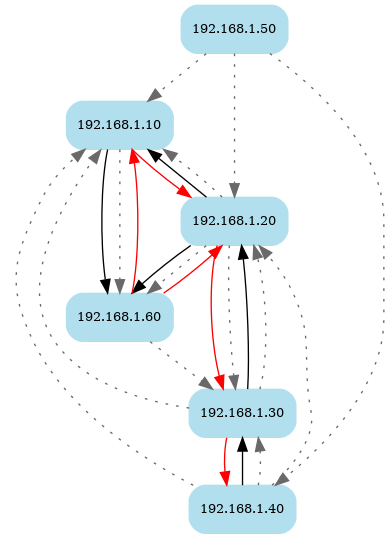
\includegraphics[scale=0.65]{chap6/network2.png}
	\caption{Simplified graph of the iTrust SWaT system network}
	\label{fig:6_network_SWaT}
\end{figure}

The graph clearly illustrates the structure of communications between the PLCs. Referring back to Table \ref{table:5_swat_ip_addresses}, which displays the IP address - PLC associations, we can observe that PLCs 1 through 4 communicate directly and sequentially with each other in a Request/Response communication pattern (represented by red and black arrows, respectively). Additionally, PLC6 communicates with both PLC1 and PLC2. On the other hand, the gray dotted arrows indicate communications for which we have knowledge of a response, but the corresponding request is unknown. For the purposes of our analysis strategy, we will not consider these communications within this context.

\bigskip
Based on our observations, the analysis strategy we will adopt involves considering sequential pairs of PLCs to effectively capture the relationships and implications between registers. %Therefore, the PLC pairs we will focus on are PLC1-2, PLC2-3, and PLC3-4. 

\section{Reverse Engineering of the iTrust SWaT System}
\label{sec:6_reverse_SWaT}
Before we delve into the analysis, it is important to provide some preliminary remarks. 

\paragraph{Analysis structure}
\label{par:6_analysis_struture}
Firstly, the analysis will be structured as a schematic analysis due to space constraints, which prevent us from presenting the extensive inferences and reasoning regarding the system in full detail. Therefore, following the analysis strategy outlined in Section \ref{sec:6_analysis_strategy}, we will concentrate exclusively on the pairs of PLCs comprising PLC1-2, PLC2-3, and PLC3-4. However, the general procedure of the methodology and how to reason about the data obtained from the framework have already been demonstrated through examples on the PLC1 of the SWaT system in Chapter \ref{chap:proposal}. We encourage readers to refer to those examples for a more comprehensive understanding. In this analysis, our focus will be on illustrating the conjectures and properties that arise from the analysis, utilizing tables and the outputs generated during the analysis.

\paragraph{Defining subsystem time duration}
\label{par:6_subsystem_duration}
The second premise addresses the process of defining the subsystems to be analyzed, which were obtained during the pre-processing phase, during the merge phase of the individual datasets. Apart from the projection determined by the considered PLCs, a time-based selection of the analysis period has also been performed (see Section \ref{subsubsec:4_select_subsystem}). This selection spans a duration of 20,000 seconds, which is equivalent to approximately five and a half hours or roughly five system cycles. The analysis begins at 100,000 seconds, which corresponds to approximately 27 hours from the start of the available data. This deliberate selection aims to exclude the initial transient period during which the SWaT system is initialized. We believe that this time range is more than sufficient for accurately defining the characteristics of the SWaT system components.

\paragraph{Conventions}
\label{par:6_conventions}
The third premise introduces a convention that governs the naming of PLC registers and will be consistently followed throughout our analysis. According to this convention, registers with similar names, such as \texttt{P1\_LIT101} and \texttt{P3\_LIT301}, \texttt{P2\_MV201} and \texttt{P3\_MV202}, are considered to belong to the \textbf{same category or type of register}. This convention allows us to establish a relationship or correspondence between registers based on their naming pattern. By grouping registers with similar names, we can infer that they serve similar functions or represent similar components in the system, such as level sensors, tanks, pumps, and so on.

\paragraph{About the Business Process Analysis}
\label{par:6_premesse_bpa}
In the end, the Business Process Analysis will focus solely on the physical process part. This is because the datasets of network traffic captures provided by iTrust for the year 2015 (as discussed in Section \ref{par:5_2015_net_dataset}) are \textbf{incomplete}. While communications related to measurements are present, those associated with actuators are entirely missing, as well as additional communications related to other system characteristics that we observed in the datasets of subsequent years. As a result, we were unable to incorporate the network event recognition component into our Business Process Analysis. To implement this component, we would require complete and overlapping network data, along with a clean physical process dataset not affected by system attacks. Unfortunately, none of the available iTrust datasets fulfill these criteria.

\subsection{Reverse Engineering of PLC1 and PLC2}
\label{subsec:6_P1P2_analysis}
The initial focus of analysis will be on the pair comprising PLC1 and PLC2. Let's delve into the main features of this subsystem by examining the outcomes obtained from applying the framework to it.

\subsubsection{Pre-processing - Preliminary Analysis}
\label{subsubsec:6_P1P2_preprocessing}

\paragraph{Measurements and Actuators Recognition} 
\label{par:6_P1P2_measures_actuators_recognition}
Listing \ref{lst:6_preproc_P1P2} shows the outcomes obtained from automatic recognition of likely measurements and actuators:

\begin{lstlisting}[language=bash, numbers=left, caption=Preliminary analysis outcomes for sensors and actuators of \texttt{PLC1-2}, label=lst:6_preproc_P1P2]
	Actuators: 
	P1_MV101 [0.0, 1.0, 2.0]
	P1_P101 [1.0, 2.0]
	P2_MV201 [0.0, 1.0, 2.0]
	P2_P203 [1.0, 2.0]
	P2_P205 [1.0, 2.0]
	
	Sensors: 
	P1_FIT101 {'max_lvl': 2.7, 'min_lvl': 0.0}
	P1_LIT101 {'max_lvl': 815.1, 'min_lvl': 489.6}
	P2_AIT201 {'max_lvl': 256.5, 'min_lvl': 252.9}
	P2_AIT202 {'max_lvl': 8.4, 'min_lvl': 8.3}
	P2_AIT203 {'max_lvl': 342.8, 'min_lvl': 320.0}
	P2_FIT201 {'max_lvl': 2.5, 'min_lvl': 0.0}
	
	Hardcoded setpoints or spare actuators: 
	P1_P102 [1.0]
	P2_P201 [1.0]
	P2_P202 [1.0]
	P2_P204 [1.0]
	P2_P206 [1.0]
\end{lstlisting}

Based on the results presented in Listing \ref{lst:6_preproc_P1P2}, the framework has identified \texttt{P1\_MV101}, \texttt{P1\_P101}, \texttt{P2\_MV201}, \texttt{P2\_P203}, and \texttt{P2\_P205} as \textbf{probable actuators}. The actuators denoted by the \textit{Pxxx} notation are binary actuators (not boolean!), meaning they have two states represented by the values 1 and 2. Conversely, the actuators identified by the \textit{MVxxx} notation are ternary actuators with three distinct states: 0, 1, and 2. 

To simplify the analysis, we have arbitrarily categorized the registers identified by the notation \textit{MVxxx} as \textbf{valves} and the registers identified by the notation \textit{Pxxx} as \textbf{pumps}. It is important to note that this distinction is solely for convenience and does \textit{not} necessarily reflect the actual role or function of these actuators within the system. 

\bigskip
\texttt{P1\_FIT101}, \texttt{P1\_LIT101}, \texttt{P2\_AIT201}, \texttt{P2\_AIT202}, \texttt{P2\_AIT203}, and \texttt{P2\_FIT201} have been identified as \textbf{likely measurements}. Upon analyzing the range of values for register \texttt{P1\_LIT101}, we observe a significant difference between the maximum and minimum values. This observation leads us to speculate that \texttt{P1\_LIT101} could be identified as a \textbf{level sensor for the tank controlled by PLC1}. However, when examining registers \texttt{P1\_FIT101}, \texttt{P2\_FIT201}, \texttt{P2\_AIT201}, and \texttt{P2\_AIT202}, the small difference between their maximum and minimum values makes it unlikely that they represent additional tanks. 

Regarding register \texttt{P2\_AIT203}, although the range of values is not as wide as in the case of \texttt{P1\_LIT101}, it is still worth examining more closely. It is possible that \texttt{P2\_AIT203} indicates the presence of a small tank. However, considering our speculation that the other \texttt{P2\_AIT20x} registers are not tank level sensors, it is uncertain whether \texttt{P2\_AIT203} falls into that category as well. Further analysis is required to confirm its role within the system.

\bigskip
Some registers have been identified as \textbf{hardcoded setpoints} or \textbf{spare actuators} based on their constant values. These registers exhibit similarities to the previously recognized pump registers. It is plausible to speculate that these registers could correspond to \textbf{spare actuators}. Moreover, the constant value of 1 associated with these registers suggests that it may represent the \textbf{OFF state} of the pumps. 

\paragraph{Actuator State Durations}
\label{par:6_P1P2_actuators_duration}
To gain a deeper understanding of the different states (0, 1, and 2) associated with valves \texttt{P1\_MV101} and \texttt{P2\_MV201}, we can analyze the duration of each state. Listing \ref{lst:6_preproc_P1P2_actuator_duration} provides information regarding the duration (in seconds) of states for these specific actuators:

\begin{lstlisting}[language=bash, numbers=left, caption=Time duration of the states of actuators \texttt{P1\_MV101} and \texttt{P1\_MV201} of PLC1-2, label=lst:6_preproc_P1P2_actuator_duration]
	Actuator state durations:
	P1_MV101 == 0.0
	9  9  10  9  9  10  9  9  10  9
	
	P1_MV101 == 1.0
	1174  1168  1182  1160  1172
	
	P1_MV101 == 2.0
	669  3019  3012  3000  2981
	
	P2_MV201 == 0.0
	8  8  8  9  9  8  9  9  9  9
	
	P2_MV201 == 1.0
	1057  1057  1045  1038  1039
	
	P2_MV201 == 2.0
	120  3135  3144  3127  3109
\end{lstlisting}

It is evident that the duration of \textbf{state 0 is relatively short}, averaging around 8-10 seconds, while the other states have much longer durations. This observation suggests that state 0 of a valve is a \textbf{transient state}, indicating a transitional phase within the valve cycle. However, without further information, it is currently not possible to determine the specific position of state 0 within the overall valve cycle.

\paragraph{Actuator State Changes}
\label{par:6_preproc_P1P2_actuator_state_changes}
Now that we have identified \texttt{P1\_LIT101} as the supposed level sensor of the tank, we can examine the trend of the tank level as the actuators change state. Listing \ref{lst:6_P1P2_preproc_changestate} provides information on the levels of the tank in correlation with the state changes of the \texttt{P1\_P101} pump:

\begin{lstlisting}[language=bash, numbers=left, caption=\texttt{P1\_P101} state changes in relation to \texttt{P1\_LIT101}, label=lst:6_P1P2_preproc_changestate]
	Actuator state changes:
	...
	P1_LIT101  P1_P101  prev_P1_P101
	 536.0356        1             2
	 533.3272        1             2
	 542.1591        1             2
	 534.8581        1             2
	 540.5890        1             2
	      ...      ...           ...
	P1_LIT101  P1_P101  prev_P1_P101
	 813.0031        2             1
	 813.0031        2             1
	 811.8256        2             1
	 812.7283        2             1
	 813.3171        2             1
	      ...      ...           ...
\end{lstlisting}

Based on the speculation that state 1 represents the OFF state of the pump and state 2 represents the ON state, we can analyze the data in Listing \ref{lst:6_P1P2_preproc_changestate}. When pump \texttt{P1\_P101} switches from the ON state to the OFF state, the average level of \texttt{P1\_LIT101} is 535. On the other hand, when \texttt{P1\_P101} goes from the OFF state to the ON state, the average level of \texttt{P1\_LIT101} is 813. These values correspond to the \textbf{minimum and maximum relative setpoints} of \texttt{P1\_P101}, respectively. 

Based on this information, we can infer that pump \texttt{P1\_P101} is responsible for \textbf{emptying the tank}. Moreover, it can be extended to assume that a pump, in general, is responsible for \textbf{water outflow}.

\bigskip
Applying the same analysis to the data for valve \texttt{P1\_MV101}, which is not reported for conciseness, we can speculate that \texttt{P1\_MV101} is responsible for \textbf{filling the tank}. In this case, states 1 and 2 would represent the \textbf{OFF and ON states of the valve}, respectively. The relative setpoints of \texttt{P1\_MV101} are approximately 500 (minimum) and 800 (maximum).
By extending this analysis, we can speculate that a valve, such as \texttt{P1\_MV101}, is responsible for controlling the \textbf{water inflow}.

\bigskip
Regarding the elements controlled by PLC2 and the sensor \texttt{P1\_FIT101}, the analysis does not reveal the presence of another tank. Therefore, we cannot determine the exact role of sensors \texttt{P2\_AIT\textit{20x}}, \texttt{P1\_FIT101} and \texttt{P2\_FIT201} at this point.
However, there is a similarity observed between the relative setpoints of \texttt{P1\_P101} and those of \texttt{P2\_MV201}, \texttt{P2\_P203}, and \texttt{P2\_P205}. These registers exhibit very similar values during state changes, suggesting a potential relationship or similar control behavior between them.

\subsubsection{Graphs and Statistical Analysis}
\label{subsubsec:6_P1P2_graphs}

\begin{figure}[ht]
	\centering
	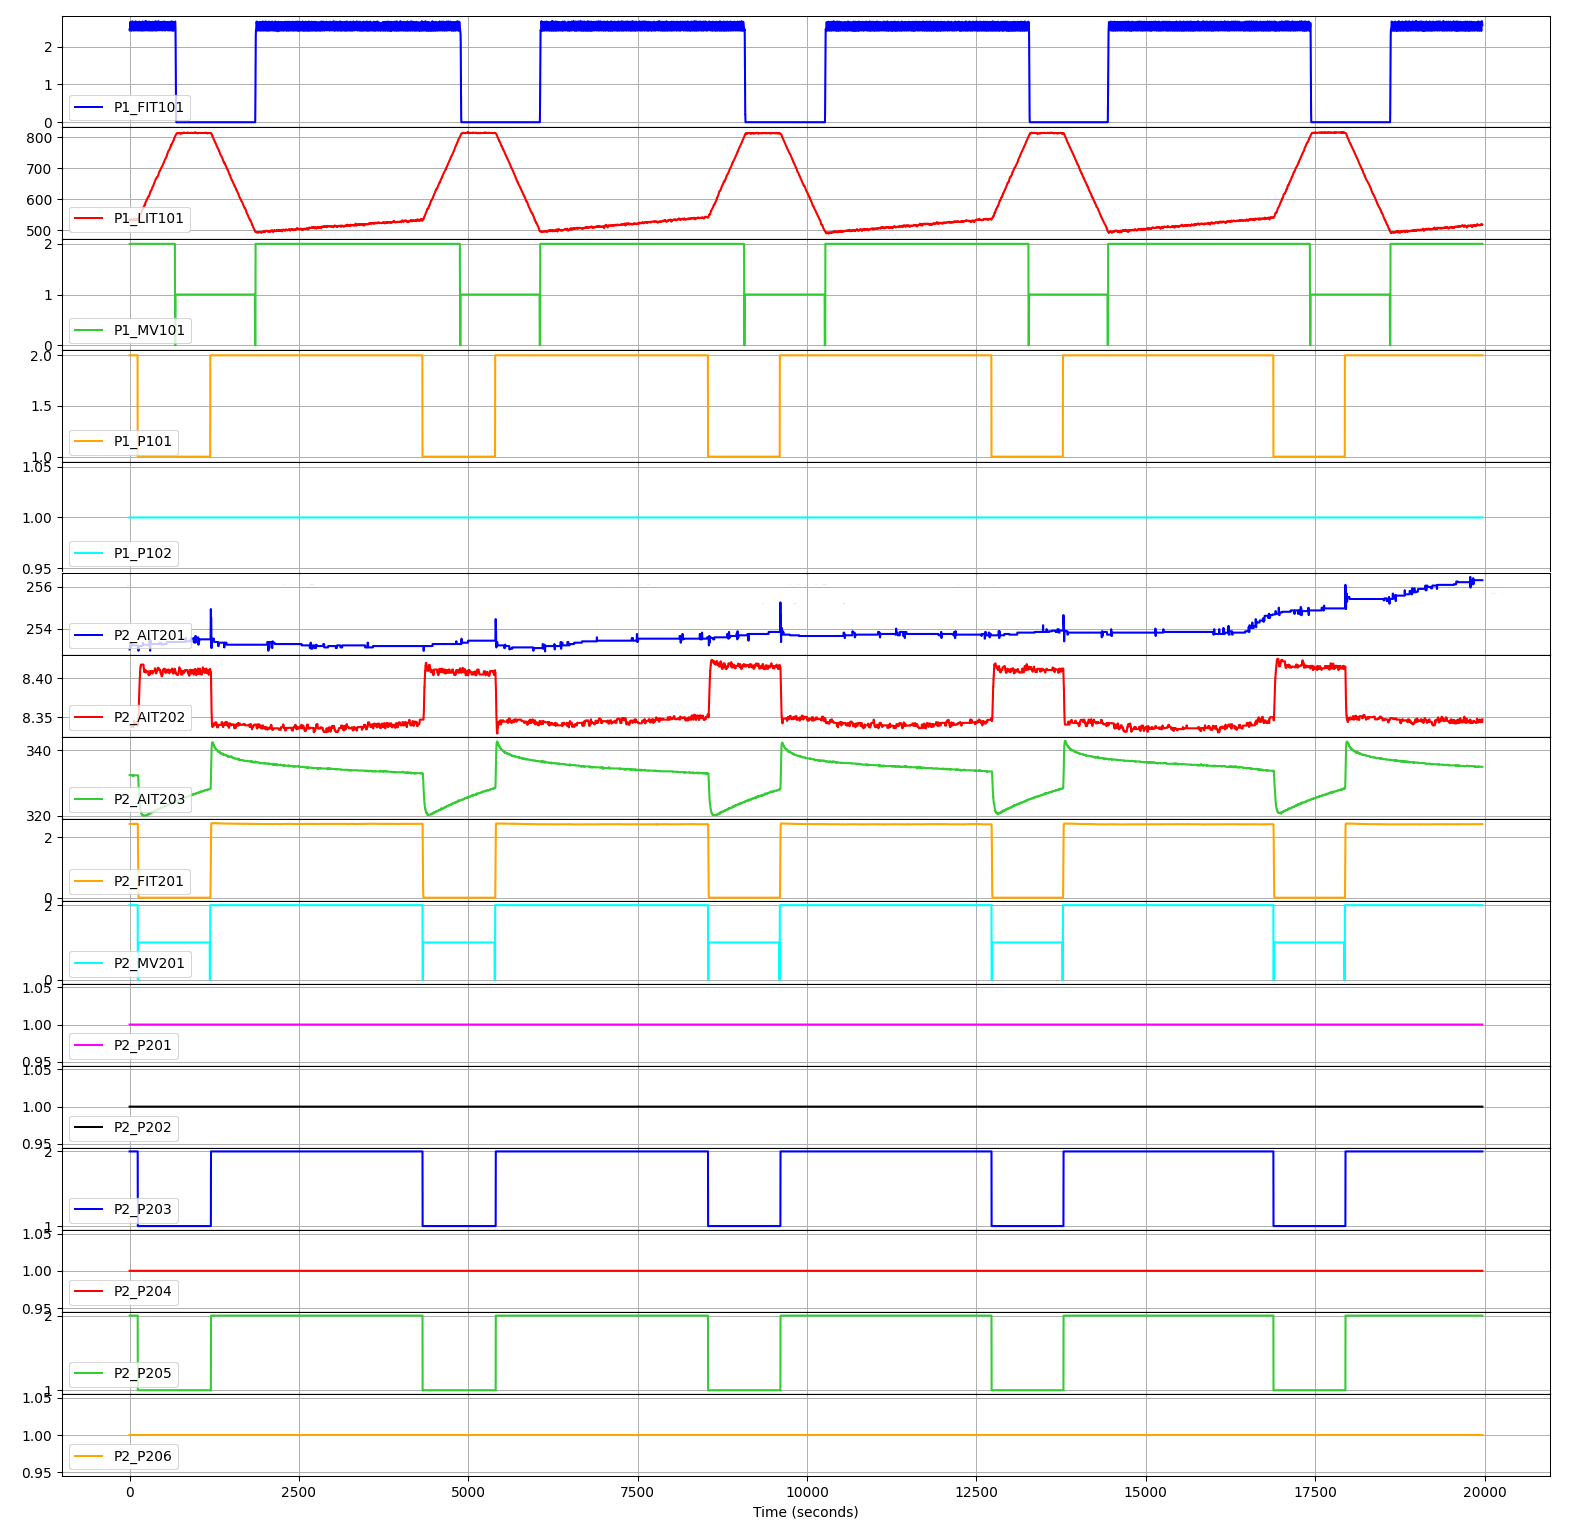
\includegraphics[scale=0.34]{chap6/P1P2_1a.png}
	\caption{Chart of PLC1-2 registers}
	\label{fig:6_P1P2_graph_full}
\end{figure}

Figure \ref{fig:6_P1P2_graph_full} illustrates the graphical representation of the registers in PLC1 and PLC2 and their respective trends.

The image provides additional support to the conjectures made during the preliminary analysis regarding the spare actuators. Furthermore, it is evident from the graphs that these spare actuators \textbf{do not appear to influence the trend} of any of the measurements. Therefore, based on this observation, we can confidently exclude these registers from further graphical analysis.

\bigskip
Figure \ref{fig:6_P1P2_graph_full_nospare} shows a clearer representation of the subsystem after removing the spare actuators.

\begin{figure}[ht]
	\centering
	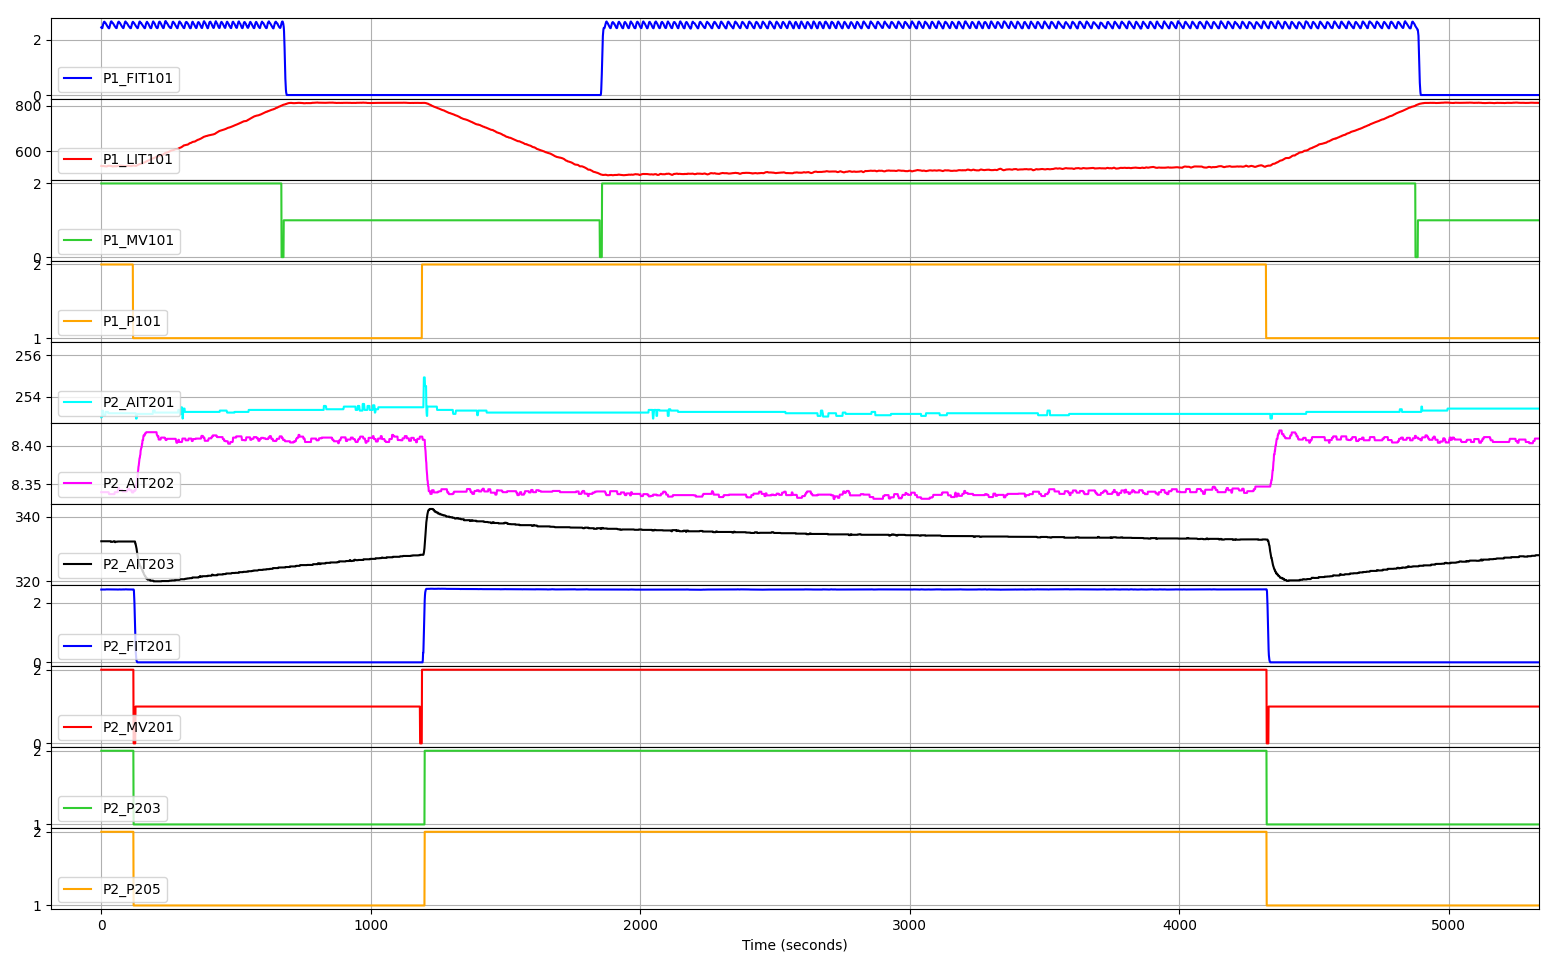
\includegraphics[scale=0.35]{chap6/P1P2_5.png}
	\caption{Chart of PLC1-2 registers without spare actuators (particular)}
	\label{fig:6_P1P2_graph_full_nospare}
\end{figure}

Figure %\ref{fig:6_P1P2_graph_full_nospare} 
provides furthermore additional insights that allow us to speculate on aspects that remained unexplained during the preliminary analysis. The most prominent aspect that stands out is the relationship between the level behavior of \texttt{P1\_LIT101} and the states of \texttt{P1\_P101} and \texttt{P1\_MV101}. It appears evident that these two actuators \textbf{do \textit{not} exhibit complementary behavior}, meaning that their states do not alternate in an \textit{ON-OFF} pattern. Instead, they can remain in the same state, either ON or OFF, for extended periods of time. When they are both in the ON state, \textbf{the growth of the tank level is slow}. However, as soon as \texttt{P1\_P101} switches to the OFF state, the tank level starts to \textbf{increase at a faster rate}. Therefore, when both of these actuators are in the ON state the influx of water into the tank exceeds the outflow of water from it. Conversely, when \texttt{P1\_MV101} switches to the OFF state, the tank level \textbf{decreases}. During periods when both actuators are in the OFF state, there is a \textit{plateau} where the tank level remains relatively \textbf{stable}.

\bigskip
Furthermore, we observe a relationship between \texttt{P1\_FIT101} and the trend of \texttt{P1\_MV101}. When the valve is in the off state, \texttt{P1\_FIT101} registers a value of 0, whereas it registers a value greater than 2 when the valve is open. This suggests that \texttt{P1\_FIT101} could be a \textbf{sensor associated with the flow} of water entering the tank, which is represented by \texttt{P1\_LIT101}. By drawing an analogy with its name, it is plausible to consider \texttt{P2\_FIT201} as another flow sensor.

\bigskip
Another intriguing aspect that arises from examining the graphs in Figure \ref{fig:6_P1P2_graph_full} and Figure \ref{fig:6_P1P2_graph_full_nospare} is the \textbf{non-cyclic pattern} observed in the \texttt{P2\_AIT201} measurement. Instead of exhibiting a cyclical trend, it follows a linear pattern. Furthermore, considering the narrow range of values associated with this measurement, it is reasonable to speculate that \texttt{P2\_AIT201} may be associated with a \textbf{sensor that measures a specific property of the water}.

The limited range of values observed in \texttt{P2\_AIT202} also raises the possibility that it functions as a sensor for a particular water characteristic, despite exhibiting a cyclic pattern. As for \texttt{P2\_AIT203}, its role remains undefined, although it also displays a cyclic trend. This trend, along with that of \texttt{P2\_AIT202}, does not appear to be related to the behavior of the valves (which rules out the possibility of it being related to a tank), but rather to that of the pumps. Consequently, it is imperative to conduct further investigations into these aspects.

\bigskip
By examining the trend of valve \texttt{P2\_MV201}, an additional speculation can be made. It appears to be independent of the trends observed in any of the measurements within this subsystem. Based on previous conjectures regarding the role of valves and considering the duration of its ON and OFF states, it is possible that \texttt{P2\_MV201} is responsible for \textbf{filling a tank that is not part of this particular subsystem}. Once again, a thorough investigation is necessary to confirm this hypothesis.

		
\subsubsection{Invariant Inference and Analysis}
\label{subsubsec:6_P1P2_invariants}
Through the process of \textit{invariant analysis}, we aim to discover new information about the system and determine whether the conjectures made in the previous steps are supported by the data obtained from the Daikon analysis.

\paragraph{General Invariants}
\label{par:6_P1P2_general_invariant}
We will begin this phase by analyzing the general invariants (see Section 4.2.5.1.). Listing \ref{lst:6_preproc_P1P2_general_invariants} presents a selection of these invariants:

\begin{lstlisting}[language=bash, numbers=left, caption=General Invariants for PLC1-2, label=lst:6_preproc_P1P2_general_invariants]
	P2_P206 == P2_P204 == P2_P202 == P2_P201 == P1_P102 == 1.0
	P2_P205 == P2_P203
	max_P1_LIT101 == 816.0
	min_P1_LIT101 == 489.0
	max_P2_AIT201 == 257.0
	min_P2_AIT201 == 252.0
	max_P2_AIT202 == 9.0
	min_P2_AIT202 == 8.0
	max_P2_AIT203 == 343.0
	min_P2_AIT203 == 320.0
\end{lstlisting}

The invariant mentioned on line 2 is particularly significant: it states that \texttt{P2\_P203} and \texttt{P2\_P205} always have the same values. While this information was somewhat apparent in the previous steps, it becomes more apparent and evident in this analysis. This observation leads us to speculate that the two pumps, \texttt{P2\_P203} and \texttt{P2\_P205}, \textbf{are related to each other} in some way. The other invariants provided in this section further reinforce the hypotheses about the spare actuators.

\vfill

\paragraph{Analysis on Single Actuator States}
\label{par:6_P1P2_single_act_states}
We proceed with the examination of the invariants derived from the \textit{first of the two semi-automatic analysis} discussed in Section \ref{par:4_single_actuator_states_analysis}. Specifically, we will focus on the analysis concerning the states of individual actuators in relation to a specific measurement, which in our case pertains to the tank represented by \texttt{P1\_LIT101}. For illustrative purposes, let's consider states 1 and 2 (OFF e ON respectively) of valve \texttt{P1\_MV101} as an example (we will disregard state 0 as it is considered transient). The conditional invariants pertinent to this scenario can be found in Listing \ref{lst:6_preproc_P1P2_conditional_invariants}.

\begin{lstlisting}[language=bash, numbers=left, caption=Conditional Invariants for states 1 and 2 of \texttt{P1\_MV101}, label=lst:6_preproc_P1P2_conditional_invariants]
	===========================
	P1_MV101 == 1.0 && P1_LIT101 < max_P1_LIT101 - 16 && P1_LIT101 > min_P1_LIT101 + 15 
	===========================
	...
	P2_P205 == P2_P203 == P2_MV201 == P1_P101 == 2.0
	P1_FIT101 == 0.0
	slope_P1_LIT101 == -1.0
	P2_FIT201 > P1_FIT101
	P2_FIT201 > P1_MV101
	P2_FIT201 > P1_P101
	...
	
	===========================
	P1_MV101 == 2.0 && P1_LIT101 < max_P1_LIT101 - 16 && P1_LIT101 > min_P1_LIT101 + 15 
	===========================
	slope_P1_LIT101 == P1_P102
	P1_FIT101 > P1_MV101
	...
	P1_MV101 >= P1_P101
	P1_MV101 >= P2_MV201
	P1_MV101 >= P2_P203
	P2_P203 >= P1_P101
	...
\end{lstlisting}

To prevent transient periods caused by water flow stabilization when the actuators change state, a condition is imposed on the level of \texttt{P1\_LIT101}. However, this condition may result in an incomplete understanding of the system's behavior. To address this, a manual refinement of the analysis is required, utilizing the \texttt{runDaikon.py} script as outlined in Section \ref{par:4_refining_analysis}.

\bigskip
Based on the analysis, the following observations can be made when the valve is in the OFF state:

\begin{itemize}
	\item The slope of \texttt{P1\_LIT101}, denoted as \texttt{slope\_P1\_LIT101}, is negative (line 7). This indicates a \textbf{downward trend} in the tank level, as we have seen in Section \ref{par:6_preproc_P1P2_actuator_state_changes}.
	\item \texttt{P1\_P101} is in state 2, or ON (line 5).
	\item \texttt{P1\_FIT101} is zero (line 6).
	\item \texttt{P2\_FIT201} has a value greater than 2 (line 10).
\end{itemize}

\noindent On the other hand, when the valve is in the ON state:

\begin{itemize}
	\item \texttt{slope\_P1\_LIT101} is positive (line 16). This indicates an \textbf{upward trend} in the tank level, as we have seen in Section \ref{par:6_preproc_P1P2_actuator_state_changes}.
	\item \texttt{P1\_FIT101} assumes a value greater than 2. The combination of this finding, along with the previous one regarding the same register, strengthens the hypothesis that this is indeed a flow sensor.
	\item \texttt{P1\_P101} can be in either the ON or OFF state, as we have seen in Section \ref{subsubsec:6_P2P3_graphs}.
\end{itemize}

When conducting a manual analysis using the \texttt{runDaikon.py} script on tank levels that fall outside the range defined by the previous condition, it does not yield useful slope information. This situation can occur because, despite the noise attenuation applied to the tank level sensor data, if there is even a single cycle in the system where the calculated slope deviates from the expected outcome, it can adversely affect the entire Daikon analysis. Figure \ref{fig:6_P1P2_slope_fail} shows this behavior.

\begin{figure}[ht]
	\centering
	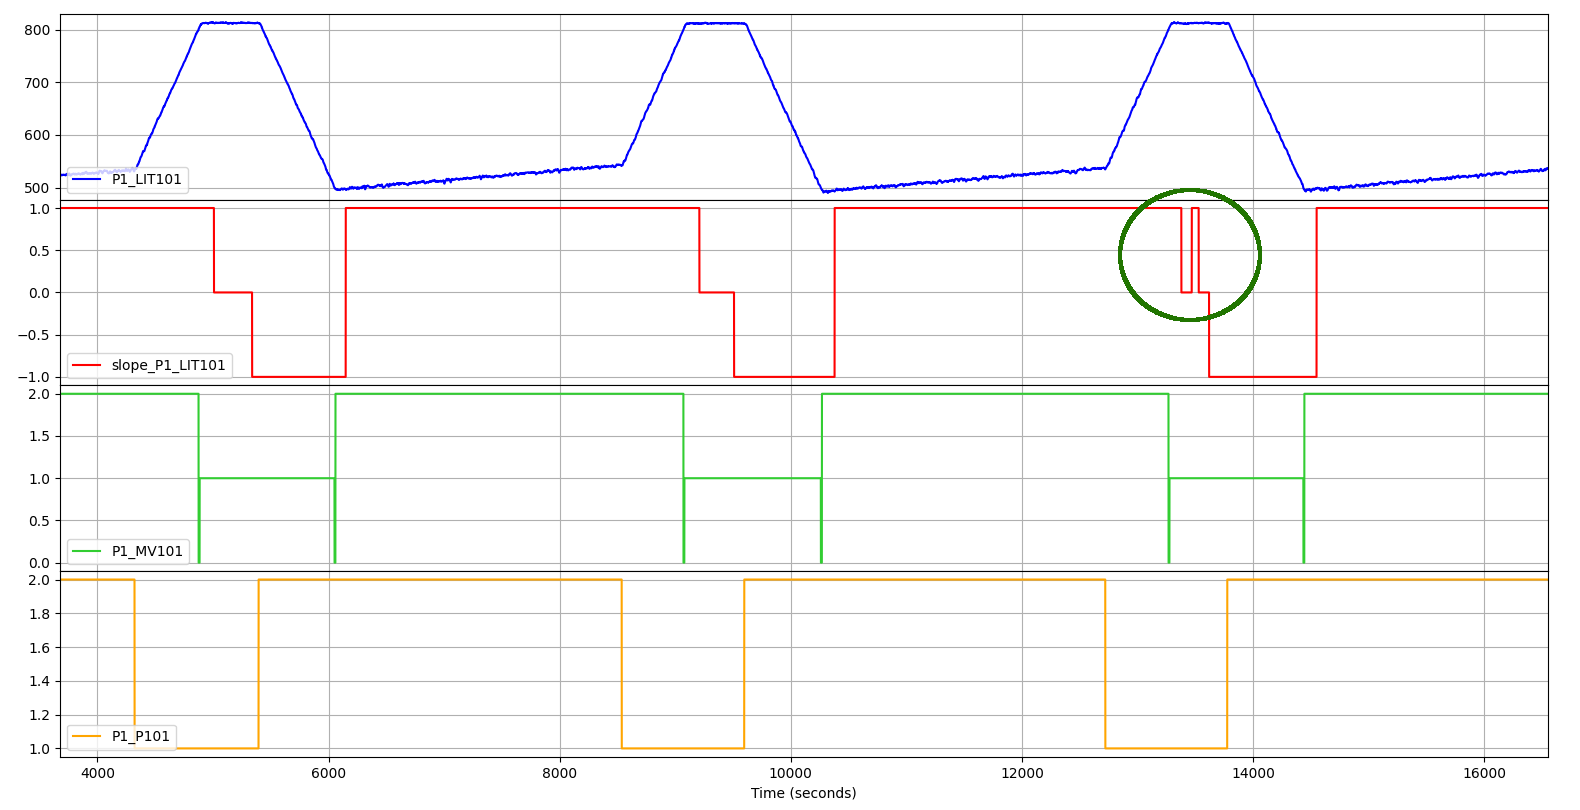
\includegraphics[scale=0.35]{chap6/P1P2_slope_error.png}
	\caption{Slope calculation anomaly (in the circle)}
	\label{fig:6_P1P2_slope_fail}
\end{figure}

\paragraph{Analysis of the Current System Configuration}
\label{par:6_P1P2_current_system_conf}
We conclude our analysis of invariants by considering the \textit{second semi-automatic analysis} outlined in Section \ref{par:4_current_system_config_analysis}, which focuses on the effective states of the system. Due to the comprehensive nature of this analysis, we will not provide a detailed report of the outputs to maintain brevity. However, this analysis confirms the findings observed in the analysis of individual actuator states. Additionally, one crucial piece of information becomes apparent for future steps: the changing state of the actuators controlled by PLC2 \textbf{do \textit{not} impact the behavior of the tank} controlled by PLC1. Indeed, it is sufficient to examine the invariant pertaining to the slope of the tank to verify this observation.


\subsubsection{Business Process Mining and Analysis}
\label{subsubsec:6_P1P2_bpa}
As explained in Section \ref{subsub:4_proc_minining_phy}, the \textit{process mining phase} applied to the physical system provides us with an immediate understanding of the system cycle and the chronological sequence of states. It enables us to determine the duration of time the system remains in a particular state and at what relative setpoint the state transition occurs concerning the reference measure. Furthermore, we can analyze the trend of this measure within each state. Additionally, we can examine the relative setpoints of other measurements to identify any connections between changes in system state and these values. 

\bigskip
Given that we have already identified the likely measurement representing the tank and the corresponding actuators that control its behavior, an activity diagram can be generated as depicted in Figure \ref{fig:6_P1P2_process_mining}.

\begin{figure}[ht]
	\centering
	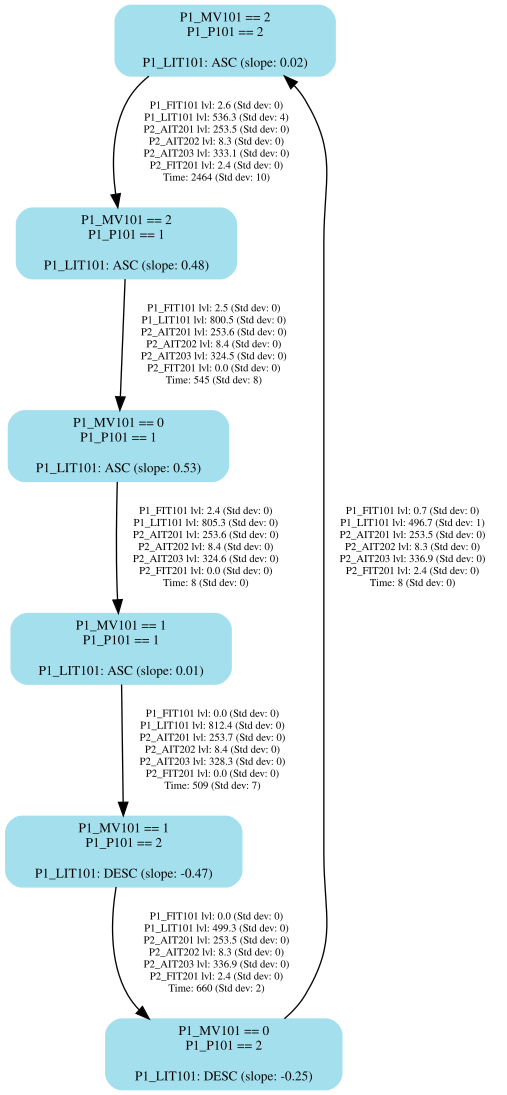
\includegraphics[scale=0.38]{chap6/business_process_P1P2.png}
	\caption{Activity diagram for PLC1-2}
	\label{fig:6_P1P2_process_mining}
\end{figure}

\bigskip
The activity diagram allows for easy interpretation of the tank level trend and slope within different states. The states where the valve has a value of 0 can be disregarded due to their short duration. Similar to the graphical analysis, there is an observed change in slope during the increasing trend of the tank level between the states \texttt{[P1\_MV101 == 2, P1\_P101 == 2]} and \texttt{[P1\_MV101 == 2, P1\_P101 == 1]}, where the slope changes from 0.02 to 0.48.

Additionally, the timing analysis on the edges reveals that the tank takes longer to fill than to empty, and the system remains in the \texttt{[P1\_MV101 == 1, P1\_P101 == 1]} state for approximately 8 minutes (509 seconds).

\bigskip
Regarding the state \texttt{[P1\_MV101 == 1, P1\_P101 == 1]}, there appears to be a discrepancy between the trend of the tank level as reported in the activity diagram and the conjectures made in the previous phases of the analysis. The activity diagram correctly depicts an increasing trend in the tank level between the end of the state \texttt{[P1\_MV101 == 2, P1\_P101 == 1]} and the end of the state \texttt{[P1\_MV101 == 1, P1\_P101 == 1]}. However, the discrepancy arises due to the fact that the interruption of flow during the valve state change from state ON to state OFF is not immediate, mainly due to the presence of the transient state 0. Additionally, water continues to flow within the piping towards the tank for a short duration even after the valve is closed. After this period, which usually lasts a few seconds, the tank level stabilizes, and there is no further inflow or outflow of water. 

By adjusting the tolerance parameter \texttt{-t} in the \texttt{processMining.py} script, it is possible to obtain accurate data regarding the behavior of the state corresponding to the \textit{plateau} observed in the graphical analysis.

\bigskip
The data presented on the arcs in the activity diagram represents the measurement values relative to the time of system state changes, specifically the relative setpoints. These values are calculated based on the average data collected in each cycle. By analyzing this data, we can observe the tank level values at which the system undergoes configuration changes and how the trend of the tank level changes accordingly. Specifically, we can see that the trend changes from ascending to stable at a tank level value of 800, from stable to descending at approximately 812, and from descending back to ascending at around 499. The change in the speed of tank filling occurs at approximately 535.

\bigskip
Furthermore, the data provides additional support for the hypothesis that the measurements associated with registers \texttt{P2\_AIT20x} are not influenced by the tank's trends.

\subsubsection{Properties}
\label{subsubsec:6_P1P2_summary_table}
From the conjectures derived from the four phases of the analysis we will derive the properties of the subsystem we are studying, which will be placed within a \textbf{summary table}. This table contains an integer identifying the property, the statement of the property itself, and from which of the four phases it was derived.

\bigskip
{\footnotesize
	\begin{longtable}[l]{p{0.05\textwidth} p{0.57\textwidth} p{0.30\textwidth}}
		\hline
		\textbf{\#} & \textbf{Statement} & \textbf{Derived from} \\
		\hline
		
		P1 & The registers \texttt{P1\_LIT101}, \texttt{P1\_FIT101}, \texttt{P2\_AIT201}, \texttt{P2\_AIT202}, \texttt{P2\_AIT203}, and \texttt{P2\_FIT201} hold likely sensor measurements. & Preliminary Analysis\newline Graphical Analysis\\
		\hline
		
		P2 & The registers \texttt{P1\_MV101}, \texttt{P1\_P101}, \texttt{P2\_MV201}, \texttt{P2\_P203}, and \texttt{P2\_P205} holds likely actuator commands. & Preliminary Analysis\newline Graphical Analysis\\
		\hline
		
		P3 & The actuators that contain the substring "MVxxx" are considered to be three-state actuators. For simplicity, we refer to them as valves. & Preliminary Analysis\\
		\hline
		
		P4 & The state 0 of these valves is associated to a transient state that occurs during the transition between state 1 (OFF) and state 2 (ON). & Preliminary Analysis\newline Graphical Analysis\\
		\hline
		
		P5 & The actuators that contain the substring "Pxxx" are considered to be binary actuators. For simplicity, we refer to them as pumps. & Preliminary Analysis \\
		\hline
		
		P6 & The registers \texttt{P1\_P102}, \texttt{P2\_P201}, \texttt{P2\_P202}, \texttt{P2\_P204}, and \texttt{P2\_P206} are associated to spare actuators. They do \textit{not} influence the trend of any measurements and they are considered in the OFF state. & Preliminary Analysis\newline Graphical Analysis\newline Invariant Analysis \\
		\hline
		
		P7 & \texttt{P1\_LIT101} is associated to the level sensor of the tank controlled by PLC1. & Preliminary Analysis\newline Graphical Analysis\\
		\hline
		
		P8 & \texttt{P1\_MV101} and \texttt{P1\_P101} are the actuators responsible for the level behavior of the water contained in the tank. & Graphical Analysis\newline Invariant Analysis\newline Business Process\\
		\hline
		
		P9 & \texttt{P1\_MV101} is responsible for filling the tank. \texttt{P1\_P101} is responsible for emptying the tank. & Graphical Analysis\newline Invariant Analysis\\
		\hline
		
		P10 & Valve are responsible for water inflow. Pumps responsible for water outflow. & Preliminary Analysis\newline Graphical Analysis\newline Invariant Analysis\\
		\hline
		
		P11 & The rate of tank level growth is slow when both \texttt{P1\_MV101} and \texttt{P1\_P101} are in the ON state. The growth speed increases when \texttt{P1\_P101} switches to the OFF state. & Graphical Analysis\newline Business Process\\
		\hline
		
		P12 & When both \texttt{P1\_MV101} and \texttt{P1\_P101} are in the ON state, the inflow of water into the tank surpasses the outflow of water from the tank. & Graphical Analysis\newline Business Process\\
		\hline
		
		P13 & The tank level decreases when \texttt{P1\_MV101} is in the OFF state and \texttt{P1\_P101} is in the ON state. & Graphical Analysis\newline Invariant Analysis\\
		\hline
		
		P14 & The tank level remains (relatively) stable when both \texttt{P1\_MV101} and \texttt{P1\_P101} are in the OFF state. & Graphical Analysis\newline Business Process\\
		\hline
		
		P15 & The trend of the tank level changes from ascending to stable when the level reaches approximately 800. It shifts from stable to descending when the level averages around 812. It changes from descending back to ascending when the level reaches about 500. The speed of tank filling increases noticeably at around 535. & Business Process \\
		\hline
		
		P16 & Absolute setpoints are 800, 812, 500 and 535. & Business Process \\
		\hline
		
		P17 & \texttt{P1\_FIT101} serves as a flow or pressure sensor to measure the inflow or the pressure of water into the tank. & Graphical Analysis\newline Invariant Analysis\newline Business Process \\
		\hline
		
		P18 & None of the actuators connected to PLC2 have an impact on the level of the tank controlled by PLC1. & Graphical Analysis\newline Invariant Analysis\newline Business Process \\
		\hline
		
		P19 & None of the measurements connected to PLC2 represent a tank. & Preliminary Analysis\newline Graphical Analysis\\
		\hline
		
		P20 & \texttt{P2\_AIT201} does not exhibit a cyclic trend. & Graphical Analysis\\
		\hline
		
		P21 & Both \texttt{P2\_AIT201} and \texttt{P2\_AIT202} serve as sensors for measuring certain properties of the water. & Preliminary Analysis\newline Graphical Analysis\\
		\hline
		
		P22 & The behavior and trend of \texttt{P2\_AIT202} and \texttt{P2\_AIT203} are directly associated with the operation of the pumps. & Graphical Analysis\newline Invariant Analysis\\
		\hline
		
		\caption{Properties of the PLC1-2 subsystem}
		\label{table:6_P1P2_summarize_properties}
	\end{longtable}
}

\subsection{Reverse Engineering of PLC2 and PLC3}
\label{subsec:6_P2P3_analysis}
Continuing our analysis of the iTrust SWaT system, our current focus will be on the registers of PLC3 and any potential relationships they may have with the registers of PLC2.

\subsubsection{Pre-processing - Preliminary Analysis}
\label{subsubsec:6_P2P3_preprocessing}

\paragraph{Measurements and Actuators Recognition}
\label{par:6_P2P3_measures_actuators_recognition}
Listing \ref{lst:6_preproc_P2P3} shows the outcomes obtained from automatic recognition of likely measurements and actuators. After previously identifying the measurements and actuators of PLC2 in Section \ref{par:6_P1P2_measures_actuators_recognition}, the listing exclusively showcases the registers associated with PLC3.

\begin{lstlisting}[language=bash, numbers=left, caption=Preliminary analysis outcomes for sensors and actuators of \texttt{PLC2-3}, label=lst:6_preproc_P2P3]
	Actuators: 
	...
	P3_MV301 [0.0, 1.0, 2.0]
	P3_MV302 [0.0, 1.0, 2.0]
	P3_MV303 [0.0, 1.0, 2.0]
	P3_MV304 [0.0, 1.0, 2.0]
	P3_P302 [1.0, 2.0]
	
	Sensors: 
	...
	P3_DPIT301 {'max_lvl': 20.4, 'min_lvl': 0.0}
	P3_FIT301 {'max_lvl': 2.4, 'min_lvl': 0.0}
	P3_LIT301 {'max_lvl': 1014.5, 'min_lvl': 786.5}
	
	Hardcoded setpoints or spare actuators: 
	...
	P3_P301 [1.0]
\end{lstlisting}

From the provided listing, it is evident that the \textbf{likely measurements} related to PLC3 are \texttt{P3\_DPIT301}, \texttt{P3\_FIT301}, and \texttt{P3\_LIT301}. Drawing an analogy with the derived properties from Table \ref{table:6_P1P2_summarize_properties}, \texttt{P3\_LIT301} can be associated with a \textbf{tank level sensor}, while \texttt{P3\_FIT301} may be linked to a flow or pressure sensor. However, the specific role of \texttt{P3\_DPIT301} cannot be speculated upon at this time.

\bigskip
Regarding the \textbf{likely actuators}, they include \texttt{P3\_MV301}, \texttt{P3\_MV302}, \texttt{P3\_MV303}, \texttt{P3\_MV304}, and \texttt{P3\_P302}. By drawing parallels with the previous analysis outcomes, it can be inferred that registers \texttt{P3\_MV30x} represent valves, while \texttt{P3\_P302} corresponds to a pump.

\bigskip
Lastly, there is a \textbf{spare actuator} identified as \texttt{P3\_P301}. Similar to the previous analysis, this is an inactive pump, indicated by the constant value of 1 in this register, signifying that it is in the OFF state.

\paragraph{Actuator State Durations}
\label{par:6_P2P3_actuators_duration}
Let's proceed with the analysis of the actuator states' duration, as displayed in Listing \ref{lst:6_preproc_P2P3_actuator_duration}. In this analysis, our focus will not be on examining the correspondence between values and the actual actuator states, as in Section \ref{par:6_P1P2_actuators_duration}. Instead, we will explore whether these actuators exhibit any distinct patterns or behaviors based on their duration.

\begin{lstlisting}[language=bash, numbers=left, caption=Time duration of the states of actuators of PLC3, label=lst:6_preproc_P2P3_actuator_duration]
	Actuator state durations:
	...
	P3_MV301 == 1.0
	2527  4154  4154  4154  4094
	
	P3_MV301 == 2.0
	36  35  36  35  34
	
	P3_MV302 == 1.0
	662  138  654  138  656  139  658  137  656  137
	
	P3_MV302 == 2.0
	62  1783  1596  1787  1591  1791  1576  1803  1540  1782
	
	P3_MV303 == 1.0
	2526  4089  4088  4089  4028
	
	P3_MV303 == 2.0
	97  96  97  96  96
		
	P3_MV304 == 1.0
	689  1832  2206  1838  2203  1840  2191  1852  2152  1831
	
	P3_MV304 == 2.0
	43  87  42  89  43  88  43  88  43  88
	
	P3_P302 == 1.0
	637  115  632  115  632  114  634  114  632  115
	
	P3_P302 == 2.0
	60  1821  1632  1825  1629  1829  1615  1841  1578  1820
\end{lstlisting}

A notable behavior is observed in the \texttt{P3\_MV30x} valves. \texttt{P3\_MV301}, \texttt{P3\_MV303}, and \texttt{P3\_MV304} have a relatively \textbf{short duration in the ON state}, ranging from around 30 seconds to a minute and a half. In contrast, \texttt{P3\_MV302} remains in the ON state for a longer duration but exhibits approximately twice as many cycles as the other actuators (10 cycles compared to 5 cycles). A similar characteristic is also observed in the OFF state of these actuators.

This behavior displayed by the actuators warrants further investigation in subsequent steps. However, based on the short duration of the ON state for \texttt{P3\_MV301}, \texttt{P3\_MV303}, and \texttt{P3\_MV304}, \textbf{it appears unlikely that they have a significant impact on the tank level}. On the other hand, the influence of \texttt{P3\_MV302} cannot be ruled out and requires additional examination.

\bigskip
We can observed that \texttt{P3\_P302}, the pump in PLC3, exhibits a behavior similar to \texttt{P3\_MV302}, with a number of cycles equal to 10. Furthermore, the durations of the ON and OFF states for both actuators appear to be overlapping. This suggests a \textbf{potential relationship between the two actuators}. Additionally, considering that \texttt{P3\_P302} is the only pump in PLC3, it is reasonable to speculate that it may have an influence on the tank level. Further investigation is necessary to validate this speculation and explore the precise nature of the relationship between \texttt{P3\_P302} and \texttt{P3\_MV302}.

\paragraph{Actuator State Changes}
\label{par:6_preproc_P2P3_actuator_state_changes}
Based on the analysis of the probable measurements, we have identified the likely tank level sensor, represented by register \texttt{P3\_LIT301}. In the previous analysis of the PLC1-2 subsystem in Section \ref{subsec:6_P1P2_analysis}, the role of valve \texttt{P2\_MV201} remained unresolved. We speculated that this actuator might be responsible for the incoming water flow to an element outside the analyzed subsystem. To investigate this further, we can examine the relationship between \texttt{P2\_MV201} and the tank within this subsystem. By extracting information from the corresponding setpoints, we can gather insights to verify if our speculation holds true. \newline 
Listing \ref{lst:6_P2P3_preproc_changestate} displays the setpoints associated with the state change of \texttt{P2\_MV201} in relation to the level of tank \texttt{P3\_LIT301}.

\begin{lstlisting}[language=bash, numbers=left, caption=\texttt{P2\_MV201} state changes in relation to \texttt{P3\_LIT301}, label=lst:6_P2P3_preproc_changestate]
	Actuator state changes:
	...
	P2_MV201  prev_P2_MV201  P3_LIT301
	       0              2  1000.2240
	       0              1   799.1140
	       0              2  1001.5060
	       0              1   799.1942
	       0              2  1001.5460
	       0              1   799.1140
	     ...            ...        ...
\end{lstlisting}

The setpoints provided in the listing support our conjecture. The maximum relative setpoint of 1000 and the minimum relative setpoint very close to 800 indicate a correlation that appears intentional. Based on this information, we can speculate that \texttt{P2\_MV201} is indeed the \textbf{valve responsible for filling the tank} associated with \texttt{P3\_LIT301}.

\bigskip
Regarding further information obtained from this step, there is limited insight available. While \texttt{P3\_P302} appears to be the pump responsible for emptying the tank associated with \texttt{P3\_LIT301}, the analysis of the actuator lifetime indicates twice as many values compared to other actuators. The pump exhibits setpoint values of approximately 850 and 970 for the transition from ON to OFF, and 900 and 1000 for the transition from OFF to ON. On the other hand, \texttt{P3\_MV302} shows numerous state changes and shares setpoints with values close to 850, 970, 1000, and 900 for the same transitions. These values align perfectly with those of the \texttt{P3\_P302} pump, suggesting a potential relationship between the two actuators.

\bigskip
Obtaining information about the remaining registers is challenging at this stage. Further analysis steps are required to gather additional insights and uncover more information about the system.

\subsubsection{Graphs and Statistical Analysis}
\label{subsubsec:6_P2P3_graphs}
Graphical analysis can provide valuable insights and help validate the conjectures made during the preliminary analysis, as well as uncover connections between registers that were not identified in the previous step. To begin, we will test the hypothesis that valve \texttt{P2\_MV201} is responsible for filling the tank associated with \texttt{P3\_LIT101}. Figure \ref{fig:6_graphs_P2P3_mv201} displays these registers, along with other registers whose behavior and relationships with the tank level we will explore in an attempt to gain a deeper understanding.

\begin{figure}[ht]
	\centering
	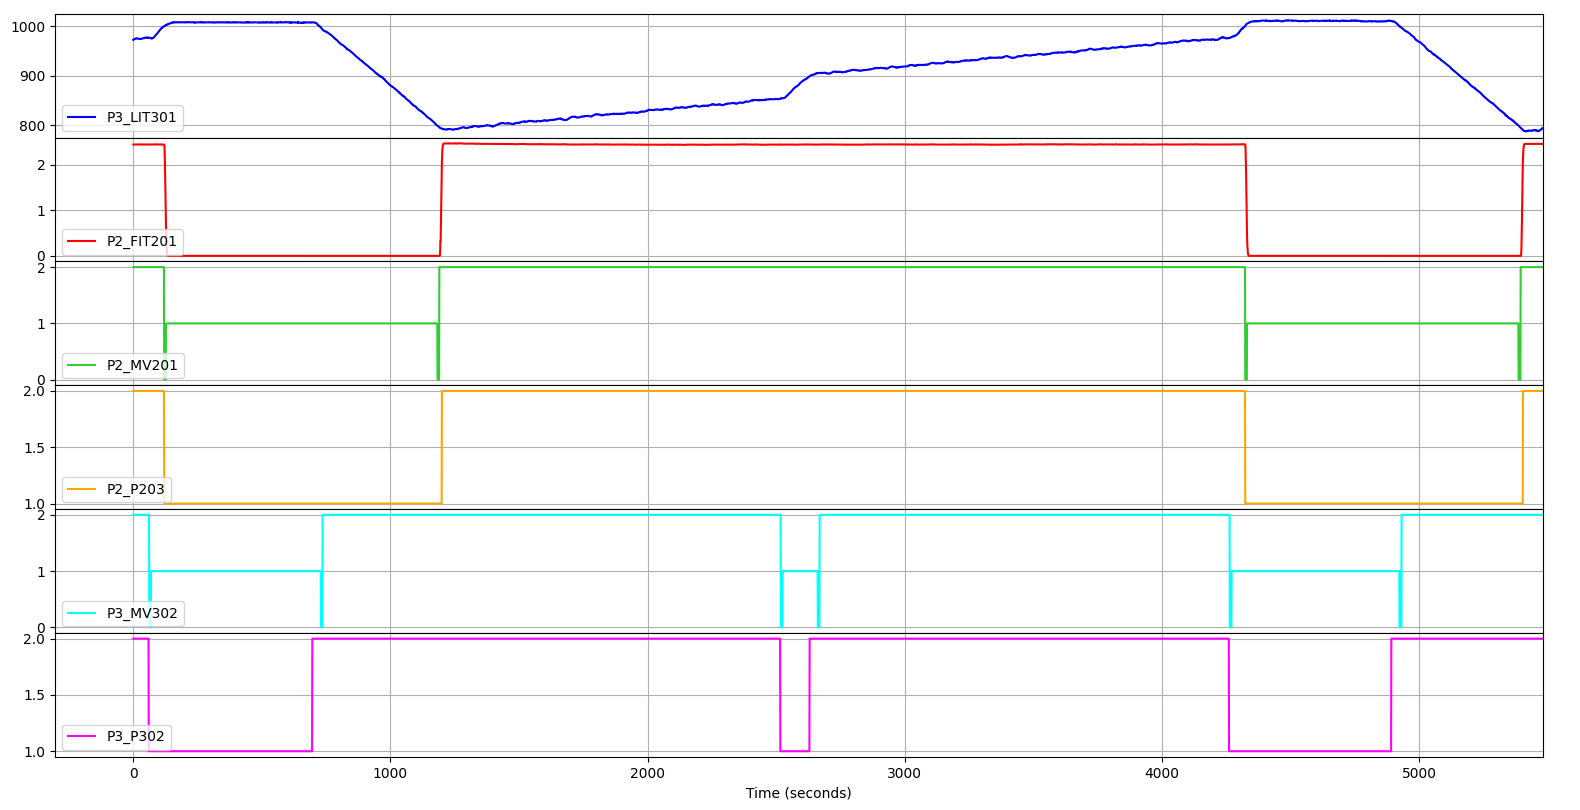
\includegraphics[scale=0.35]{chap6/P2P3_7.png}
	\caption{Verifying the conjecture about valve \texttt{P2\_MV201} }
	\label{fig:6_graphs_P2P3_mv201}
\end{figure}

\bigskip
Figure \ref{fig:6_graphs_P2P3_mv201} shows the particular behavior of \texttt{P3\_LIT103}, with two slope changes during the tank filling period. These slope changes correspond approximately to the relative setpoints found for \texttt{P3\_MV302} and \texttt{P3\_P302}. However, we will analyze this aspect later.
What we can see in relation to the initial conjecture about the role of \texttt{P2\_MV201} is that the period during which the valve remains in the ON state corresponds exactly to the increasing trend of \texttt{P3\_LIT301}. The conjecture thus finds further support. We also note how \texttt{P2\_FIT201} is related to the trend of \texttt{P2\_MV201} and the increasing trend of \texttt{P3\_LIT301}. 

\bigskip
Now let's examine the relationships between the tank represented by \texttt{P3\_LIT301} and the other actuators of PLC3 through Figure \ref{fig:6_graphs_P3}.

\begin{figure}[ht]
	\centering
	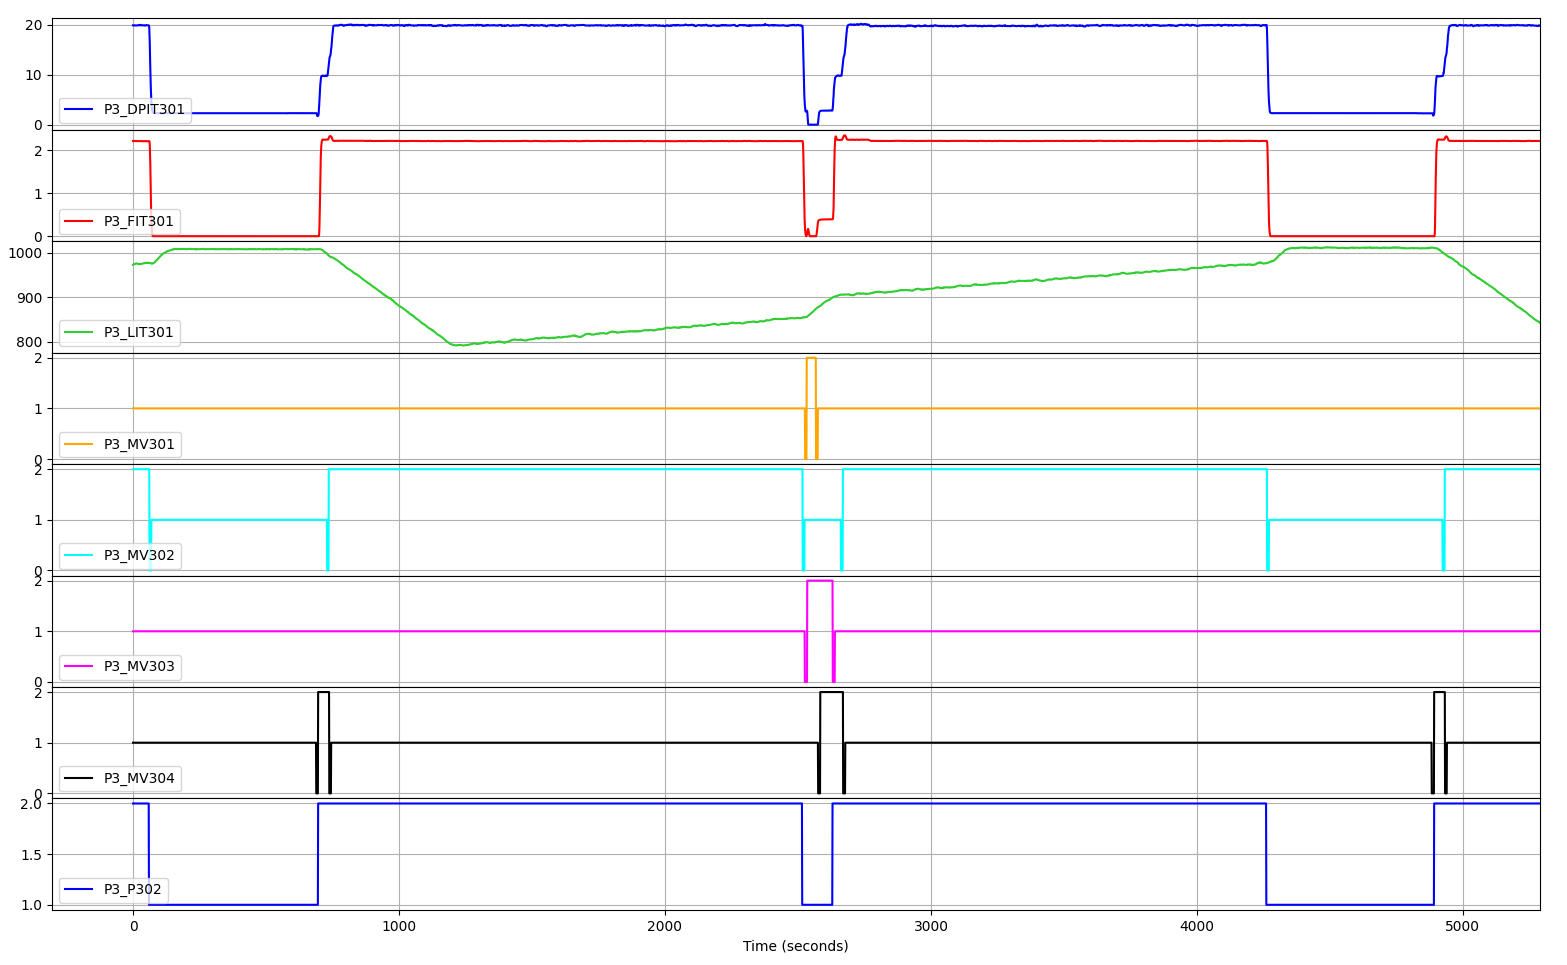
\includegraphics[scale=0.35]{chap6/P3_3.png}
	\caption{PLC3 registers}
	\label{fig:6_graphs_P3}
\end{figure}

From the charts, it is evident that the trends of \texttt{P3\_DPIT301} and \texttt{P3\_FIT301} exhibit similarities. Furthermore, their overall pattern closely follows that of the valve \texttt{P3\_MV302}. Based on these observations, we can speculate that there is a relationship between these registers or that they serve similar functions, possibly as p\textbf{ressure or flow sensors}.

\bigskip
Regarding pump \texttt{P3\_P302}, we observe that its OFF state coincides with the increasing slope of P3\_LIT301 during its upward trend and the entire phase when the level remains relatively stable. Conversely, its ON state corresponds to the gradual increase and decrease of the water level in the tank. This observation provides further evidence to support the hypothesis that \texttt{P3\_P302} is responsible for emptying the tank.

Valve \texttt{P3\_MV302} exhibits a similar pattern to pump \texttt{P3\_P302}. Building upon our previous findings, we can speculate that, similar to \texttt{P2\_MV201} in the previous analyzed subsystem, \texttt{P3\_MV302} is responsible for controlling the incoming flow to another element outside the analyzed subsystem.

\bigskip
Let us now analyze the potential roles of valves \texttt{P3\_MV301}, \texttt{P3\_MV303}, and \texttt{P3\_MV304} in relation to the indicated tank level. It seems unlikely that \texttt{P3\_MV304} has any direct impact on the tank level. The valve is activated twice within one system cycle, but there are no noticeable changes in \texttt{P3\_LIT301} during its first opening. This suggests that the second opening is also insignificant in terms of tank level. However, it is worth noting the slight peaks in \texttt{P3\_FIT301} that occur shortly after the valve's opening.

Regarding the remaining valves, \texttt{P3\_MV301} and \texttt{P3\_MV303}, their impact on the tank level is still unclear, particularly during the increased slope of \texttt{P3\_LIT101} around the second 2500. Figure \ref{fig:6_graphs_P3_zoom}  provides us with a comprehensive overview of the situation.

\vfill
\pagebreak
\begin{figure}[H]
	\centering
	\begin{subfigure}{0.90\textwidth}
		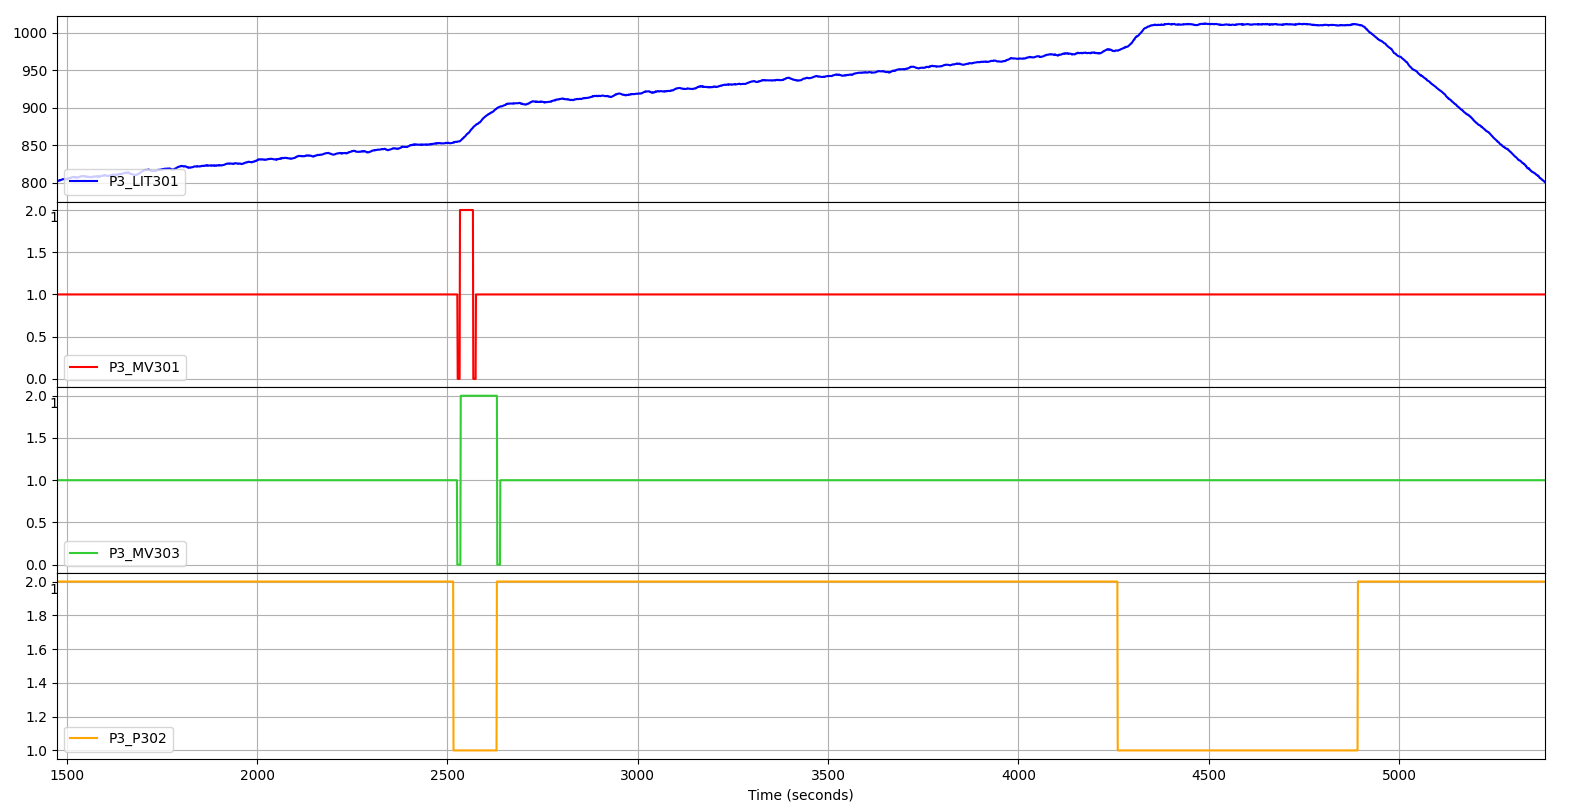
\includegraphics[width=\textwidth]{chap6/P3_8.png}
		\caption{}
		\label{subfig:6_mv301}
	\end{subfigure}
%\end{figure}
%\begin{figure}[H]\ContinuedFloat
	\begin{subfigure}{0.90\textwidth}
		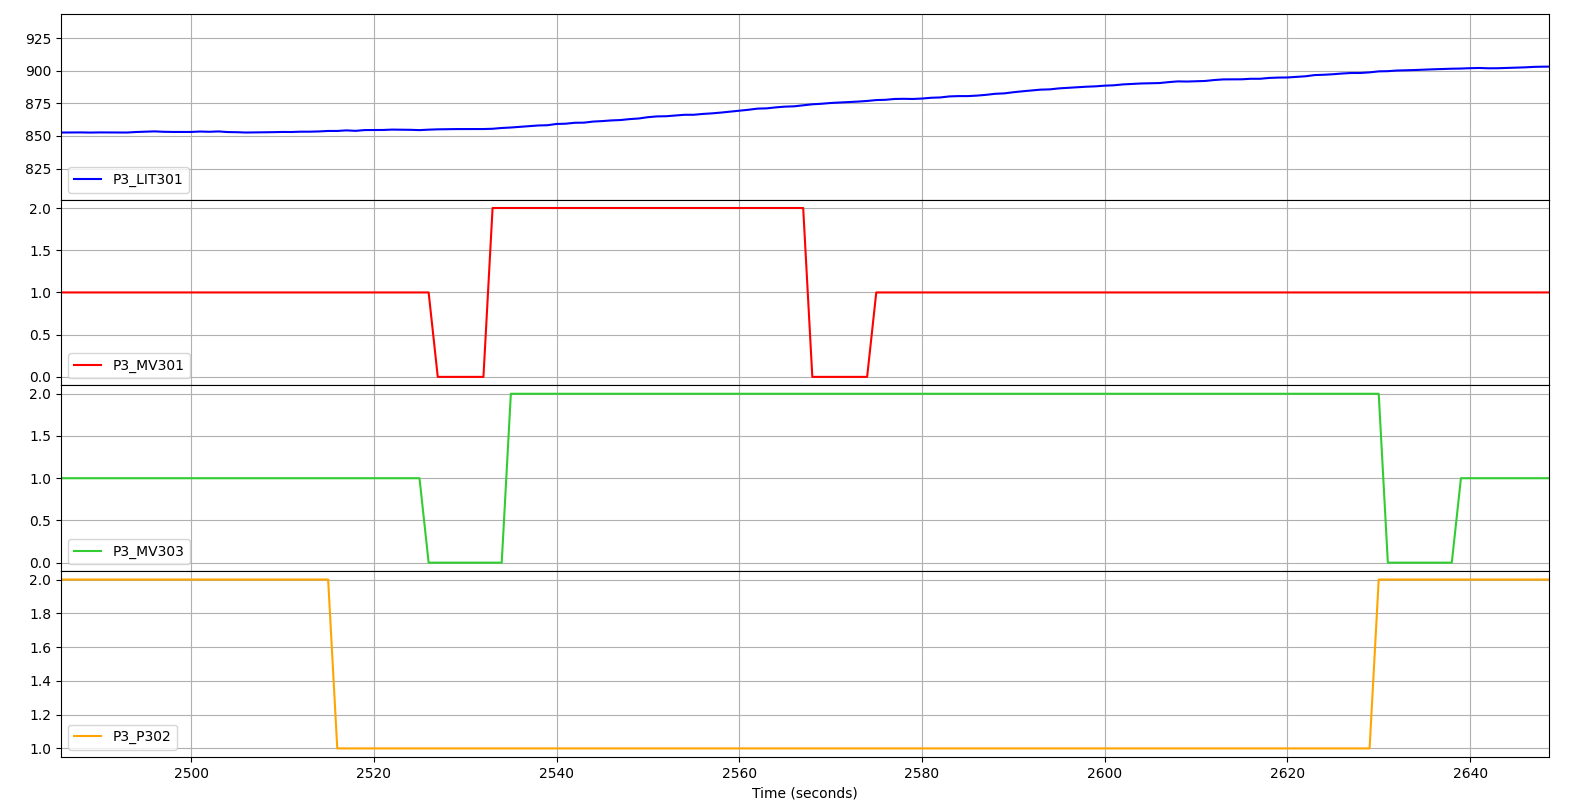
\includegraphics[width=\textwidth]{chap6/P3_8b.png}
		\caption{}
		\label{subfig:6_mv301_zoom}
	\end{subfigure}
	\caption{\texttt{P3\_MV301} and \texttt{P3\_MV303} analysis}
	\label{fig:6_graphs_P3_zoom}
\end{figure}

The analysis of the valves \texttt{P3\_MV301} and \texttt{P3\_MV303} indeed presents some challenges. However, upon closer examination of Figure \ref{subfig:6_mv301_zoom}, we observe that when these valves are in the ON state, the slope of \texttt{P3\_LIT301} remains relatively constant. This is unexpected, as one would anticipate a steeper slope due to the inflow of liquid. Additionally, in Figure \ref{subfig:6_mv301}, we can observe that when these valves are in the OFF state, the slope of \texttt{P3\_LIT301} from the second 4300 remains similar to the section we are currently analyzing. Based on these observations, we speculate that these valves either \textbf{do not affect the water level of the tank} or have a minimal, undetectable impact.

\bigskip
Indeed, Figure \ref{fig:6_graphs_P3} provides additional insights into the relationship between the valves \texttt{P3\_MV301}, \texttt{P3\_MV303}, and \texttt{P3\_MV304} and the sensors \texttt{P3\_DPIT301} and \texttt{P3\_FIT301}. The graph shows that the values of \texttt{P3\_DPIT301} and \texttt{P3\_FIT301} undergo noticeable changes during the activation of these valves, suggesting a potential connection between them. This observation supports the hypothesis that the valves and sensors are linked in some way.

\subsubsection{Invariant Inference and Analysis}
\label{subsubsec:6_P2P3_invariants}

\paragraph{General Invariants}
\label{par:6_P2P3_general_invariant}

The analysis of general invariants does not yield any significant insights. However, it confirms the maximum and minimum values of the measurements seen in Section \ref{par:6_P2P3_measures_actuators_recognition} and identifies the presence of the spare actuator \texttt{P3\_P301}. 

\paragraph{Analysis on Single Actuator States}
\label{par:6_P2P3_single_act_states}
The analysis of single actuator states reveals additional information. The resulting invariants provide further support for the conjecture regarding the roles of \texttt{P2\_MV201} and \texttt{P3\_P302} in regulating the water level in the tank, with the former responsible for filling and the latter for emptying. Listing \ref{lst:6_preproc_P2P3_conditional_invariants} presents the specific invariants involved in this analysis.

\begin{lstlisting}[language=bash, numbers=left, caption=Conditional Invariants for \texttt{P2\_MV201} and \texttt{P3\_P302}, label=lst:6_preproc_P2P3_conditional_invariants]
	===========================
	P2_MV201 == 1.0 && P3_LIT301 < max_P3_LIT301 - 20 && P3_LIT301 > min_P3_LIT301 + 24 
	===========================
	P3_P301 == P3_MV303 == P3_MV301 == P2_P205 == P2_P203 == P2_MV201 == 1.0
	P3_P302 == 2.0
	slope_P3_LIT301 == -1.0
	P3_FIT301 > P2_MV201
	P3_DPIT301 > P3_FIT301 > P3_P302
	...
	===========================
	P2_MV201 == 2.0 && P3_LIT301 < max_P3_LIT301 - 20 && P3_LIT301 > min_P3_LIT301 + 24 
	===========================
	P2_P205 == P2_P203 == P2_MV201 == 2.0
	slope_P3_LIT301 == P2_P201
	P2_FIT201 > P2_MV201
	P2_FIT201 > P2_P201
	P2_FIT201 > P3_FIT301
	...
	===========================
	P3_P302 == 1.0 && P3_LIT301 < max_P3_LIT301 - 20 && P3_LIT301 > min_P3_LIT301 + 24 
	===========================
	P2_P205 == P2_P203 == P2_MV201 == 2.0
	slope_P3_LIT301 == P3_P302 == P2_P201
	P2_FIT201 > P2_MV201
	P2_FIT201 > P3_FIT301
	...
	===========================
	P3_P302 == 2.0 && P3_LIT301 < max_P3_LIT301 - 20 && P3_LIT301 > min_P3_LIT301 + 24 
	===========================
	P2_MV201 one of { 1.0, 2.0 }
	slope_P3_LIT301 one of { -1.0, 1.0 }
	P3_DPIT301 > P3_P302 > slope_P3_LIT301
	...
\end{lstlisting}

Moreover, from the analysis of the invariants it becomes apparent that when \texttt{P3\_P302} is in the ON state and \texttt{P2\_MV201} is in the OFF state, both \texttt{P3\_FIT301} and \texttt{P3\_DPIT301} take values greater than 2 (as derived from lines 5, 7, 8 and 32 of the listing). 

\bigskip
Regarding the valves \texttt{P3\_MV301} and \texttt{P3\_MV303}, Daikon's analysis does not provide specific information about their behavior during changes in slope when the water level rises. Therefore, further analysis is required to understand their role in the system.

However, one observation can be made regarding \texttt{P3\_MV304}. Daikon's analysis reveals two different slopes (increasing and decreasing) when this valve is in the ON state, which aligns with the observations made in the Graphical Analysis in Section \ref{subsubsec:6_P2P3_graphs}. This finding strengthens the conecture that \texttt{P3\_MV304} does not play a significant role in the tank cycle represented by \texttt{P3\_LIT301}.

\paragraph{Analysis of the Current System Configuration}
\label{par:6_P2P3_current_system_conf}
To simplify the analysis and facilitate the interpretation of outcomes, two separate groups of actuators were analyzed. The first group consists of \texttt{P2\_MV201} and \texttt{P3\_P302}, which are conjectured to regulate the level of the tank. The second group includes \texttt{P3\_MV301}, \texttt{P3\_MV303}, and \texttt{P3\_MV304}, for which it is speculated that they do not play a role in regulating the tank level. This grouping allows for a clearer examination of the states of the system and provides an opportunity to gain a better understanding of the behavior of these actuators. By analyzing these two groups separately, it becomes easier to draw conclusions and make comparisons between the different sets of actuators.

\bigskip
The analysis of the first group of actuators, specifically \texttt{P2\_MV201} and \texttt{P3\_P302}, further supports the conjectures made regarding their behavior in relation to the trend of the tank level. It was necessary to refine the analysis manually using the \texttt{runDaikon.py} script to obtain more detailed insights, particularly for the state \texttt{[P2\_MV201 == 2, P3\_P302 == 2]}. 

Regarding the second group of actuators, the analysis of their states only reinforces the hypothesis that their activation does not have a significant impact on the trend of tank level represented by \texttt{P3\_LIT301}. 

\bigskip
Unfortunately, no further useful information can be derived from this phase of the analysis. To address the remaining questions and clarify any outstanding issues, we will proceed to the next and final phase of the subsystem analysis.

\vfill

\subsubsection{Business Process Mining and Analysis}
\label{subsubsec:6_P2P3_bpa}

One of the hypotheses that needed to be tested was whether the valves \texttt{P3\_MV301}, \texttt{P3\_MV303}, and \texttt{P3\_MV304} have an impact on the tank level in the section between setpoints 850 and 900. Our initial assumption was that these actuators do not affect the level detected by \texttt{P3\_LIT301} because, as observed in the Graphical Analysis, the slope in that interval is similar to the slope between setpoints 970 and 1000, where these valves are not involved.

To verify this conjecture, we utilized the JSON file generated by the \texttt{processMining.py} script. This script allows us to isolate the specific intervals and calculate the slope for each of them. In Listing \ref{lst:6_preproc_P2P3_bp1}, we present the outcomes of these calculations, providing further insights into the behavior of the valves during those intervals.

\begin{lstlisting}[language=bash, numbers=left, caption=Slope calculation of \texttt{P3\_LIT301} for the 850-900 and 970-1000 intervals related to tank levels, label=lst:6_preproc_P2P3_bp1]
	"slope_P3_LIT301": [
	0.383, # from 970 to 1000
	0.395, # from 850 to 900
	0.384,
	0.395,
	0.354,
	0.38,
	0.388,
	0.381,
	0.385,
	0.386
	],
\end{lstlisting}

The provided data in Listing \ref{lst:6_preproc_P2P3_bp1} illustrates the calculated slopes for the intervals between 970 and 1000 (odd-numbered lines) and the intervals between 850 and 900 (even-numbered lines). Upon examination, we observe that the values for these two intervals are nearly identical, accounting for some expected fluctuations. This finding reinforces our initial conjecture that the \texttt{P3\_MV301}, \texttt{P3\_MV303} and \texttt{P3\_MV304} valves do not play a role in the process of filling and emptying the tank. It is indeed possible to speculate that the \texttt{P3\_MV30x} valves, similar to \texttt{P3\_MV302}, might have a role in a different part of the system that has not been analyzed in the current context. 

\bigskip
Based on the activity diagram obtained from the analysis of actuators \texttt{P2\_MV201} and \texttt{P3\_P302} (Figure \ref{fig:6_P2P3_process_mining}), the behavior of subsystem PLC2-3 can be summarized as follows:

\begin{itemize}
	\item When the system is in the states \texttt{[P2\_MV201 == 2, P3\_P302 == 2]} and \texttt{[P2\_MV201 == 2, P3\_P302 == 1]}, the level of the tank represented by \texttt{P3\_LIT301} is increasing. The tank level exhibits a faster growth rate in the latter state.
	
	\item When the system is in the state \texttt{[P2\_MV201 == 1, P3\_P302 == 1]}, the tank level remains stable.
	
	\item When the system is in the state \texttt{[P2\_MV201 == 1, P3\_P302 == 2]}, the tank level is decreasing.
\end{itemize}

The \textbf{absolute setpoints} for the tank level in subsystem PLC2-3 are defined as follows: the minimum setpoint is 800, the maximum setpoint is 1000, and there are additional setpoints at 850, 900, and 970, which correspond to specific changes in the slope of the tank level.

\bigskip
Taking a closer look at the behavior of sensors \texttt{P2\_FIT201} and \texttt{P3\_FIT301}, we observe the following patterns: \texttt{P2\_FIT201}, which is associated with incoming water flow and connected to valve \texttt{P2\_MV201}, exhibits values greater than 2 when the valve is in the ON state. Conversely, when the valve is set to OFF, the sensor reading drops to 0.

Regarding \texttt{P3\_FIT301}, it appears to be linked to the behavior of the pump \texttt{P3\_P301} and correlates with the water flow out of the tank. When the pump is activated and in the ON state, the sensor records values greater than 2. On the other hand, when the pump is turned off and in the OFF state, the sensor reading returns to 0.

\pagebreak
%\begin{comment}
\begin{figure}[H]
	\centering
	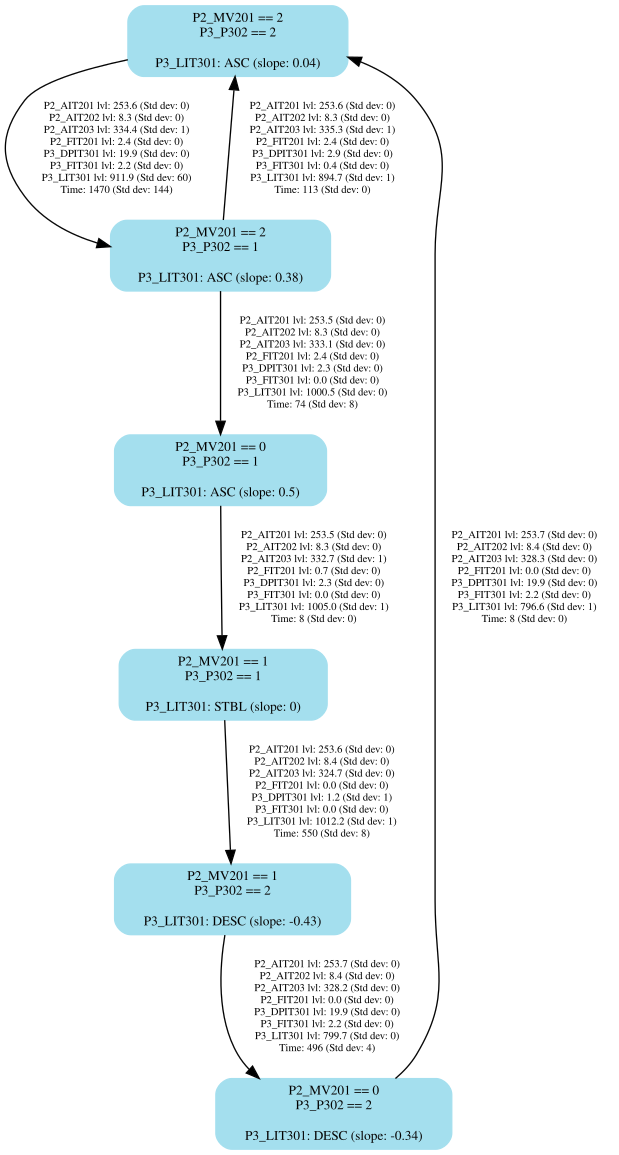
\includegraphics[scale=0.48]{chap6/business_process_P2P3a.png}
	\caption{Activity diagram for PLC2-3}
	\label{fig:6_P2P3_process_mining}
\end{figure}
%\end{comment}
\pagebreak

\vfill

\subsubsection{Properties}
\label{subsubsec:6_P2P3_summary_table}
Table \ref{table:6_P2P3_summarize_properties} provides a summary of the properties inferred from the conjectures made throughout the different stages of the analysis.

\bigskip
{\footnotesize
	\begin{longtable}[l]{p{0.05\textwidth} p{0.57\textwidth} p{0.30\textwidth}}
		\hline
		\textbf{\#} & \textbf{Statement} & \textbf{Derived from} \\
		\hline
		
		P23 & The registers \texttt{P3\_DPIT301}, \texttt{P3\_FIT301}, and \texttt{P3\_LIT301} of PLC3 hold likely sensor measurements. & Preliminary Analysis\newline Graphical Analysis \\
		\hline
		
		P24 & The registers \texttt{P3\_MV301}, \texttt{P3\_MV302}, \texttt{P3\_MV303}, \texttt{P3\_MV304}, and \texttt{P3\_P302} of PLC3 hold likely actuator commands. & Preliminary Analysis\newline Graphical Analysis \\
		\hline
		
		P25 & The register \texttt{P3\_P301} of PLC3 is associated to a spare actuator. & Preliminary Analysis\newline Graphical Analysis\newline Invariant Analysis \\
		\hline
		
		P26 & The register \texttt{P3\_LIT301} of PLC3 is associated to the level sensor of the tank controlled by PLC3. & Preliminary Analysis\newline Graphical Analysis \\
		\hline
		
		P27 & \texttt{P2\_MV201} and \texttt{P3\_P302} are are associated to the actuators responsible for the level behavior of the water contained in the tank. & Graphical Analysis\newline Invariant Analysis\newline Business Process \\
		\hline
		
		P28 & The rate of tank level growth is slow when both \texttt{P2\_MV201} and \texttt{P3\_P302} are in the ON state. The growth speed increases when \texttt{P3\_P302} switches to the OFF state. & Graphical Analysis\newline Business Process \\
		\hline
		
		P29 & When both \texttt{P2\_MV201} and \texttt{P3\_P302} are in the ON state, the inflow of water into the tank surpasses the outflow of water from the tank. & Graphical Analysis\newline Business Process \\
		\hline
		
		P30 & The tank level decreases when \texttt{P2\_MV201} is in the OFF state and \texttt{P3\_P302} is in the ON state. & Graphical Analysis\newline Invariant Analysis \\
		\hline
		
		P31 & The tank level remains (relatively) stable when both \texttt{P2\_MV201} and \texttt{P3\_P302} are in the OFF state. & Graphical Analysis\newline Business Process \\
		\hline
		
		P32 & The trend of the tank level switches from ascending to stable when the level reaches approximately 1000. It shifts from stable to descending when the level averages around 1012. It changes from descending back to ascending when the level reaches about 800. The slope of thank filling increases noticeably from around 850 to 900 and from around 970 to 1000. & Business Process \\
		\hline
		
		P33 & Absolute setpoints are 800, 850, 900, 970, 1000. & Business Process \\
		\hline
		
		P34 & \texttt{P2\_FIT201} is associated to a flow or pressure sensor to the \texttt{P3\_LIT301} register. It is related to the \texttt{P2\_MV201} valve. & Graphical Analysis\newline Invariant Analysis\newline Business Process\\
		\hline
		
		P35 & \texttt{P3\_FIT301} and \texttt{P3\_DPIT301} exhibit similar patterns in their behavior. Both registers are related to the operation of pump \texttt{P3\_P302} and, consequently, to the flow of water out of the tank. & Graphical Analysis\newline Business Process \\
		\hline
		
		P36 & The registers \texttt{P3\_MV301}, \texttt{P3\_MV303}, and \texttt{P3\_MV304} do not have an impact on the water level dynamics of the tank controlled by PLC3. & Graphical Analysis\newline Business Process \\
		\hline
		
		\caption{Properties of the PLC2-3 subsystem}
		\label{table:6_P2P3_summarize_properties}
	\end{longtable}
}

\subsection{Reverse Engineering of PLC3 and PLC4}
\label{subsec:6_P3P4_analysis}
In the final phase of the reverse engineering process, the focus is directed towards the subsystem consisting of PLC3 and PLC4 in the iTrust SWaT system. Given the constraints of the thesis, this section will provide a concise and schematic overview compared to the earlier sections.

\subsubsection{Pre-processing - Preliminary Analysis}
\label{subsubsec:6_P3P4_preprocessing}

\paragraph{Measurements and Actuators Recognition}
\label{par:6_P3P4_measures_actuators_recognition}

Listing \ref{lst:6_preproc_P3P4} shows the outcomes obtained from automatic recognition of likely measurements and actuators for PLC4. We omit those related to PLC3 as they are already known.

\begin{lstlisting}[language=bash, numbers=left, caption=Preliminary analysis outcomes for sensors and actuators of \texttt{PLC3-4}, label=lst:6_preproc_P3P4]
	Actuators: 
	...
	
	Sensors: 
	...
	P4_AIT401 {'max_lvl': 148.8, 'min_lvl': 148.8}
	P4_AIT402 {'max_lvl': 191.1, 'min_lvl': 185.5}
	P4_FIT401 {'max_lvl': 1.7, 'min_lvl': 1.7}
	P4_LIT401 {'max_lvl': 1002.8, 'min_lvl': 775.8}
	
	Hardcoded setpoints or spare actuators: 
	...
	P4_P401 [1.0]
	P4_P402 [2.0]
	P4_P403 [1.0]
	P4_P404 [1.0]
	P4_UV401 [2.0]
\end{lstlisting}

From the information provided in Listing \ref{lst:6_preproc_P3P4}, several observations can be made. Firstly, it is noted that there are no apparent actuators listed in the analysis. The likely sensors identified include \texttt{P4\_AIT401}, \texttt{P4\_AIT402}, \texttt{P4\_FIT401}, and \texttt{P4\_LIT401}. Among these sensors, \texttt{P4\_LIT401} is presumed to be the level sensor for the tank controlled by PLC4 based on similarities with the previous cases.

\bigskip
It is acknowledged that \texttt{P4\_FIT401} and \texttt{P4\_AIT401} are recognized as sensors, despite their seemingly constant values. It is important to note that the script used to identify likely actuators and sensors rounds the values to the first decimal place. Therefore, it is inferred that these registers contain continuous data with narrow value ranges.

Drawing on the analogy with the P21 property mentioned in Section \ref{subsubsec:6_P1P2_summary_table}, it is speculated that the \texttt{P4\_AIT40x} registers represent measurements related to some water property. Additionally, \texttt{P4\_FIT401} is speculated to represent a pressure or flow sensor, based on similarities observed in previous cases.

\bigskip
In the analysis of the hardcoded setpoints and spare actuators, two registers stand out: \texttt{P4\_P402} and \texttt{P4\_UV401}, both with a value of 2. Drawing on analogies from previous cases, \texttt{P4\_P402} is speculated to represent a pump that is constantly in the ON state and therefore active. However, regarding \texttt{P4\_UV401}, it is unclear whether it is an actuator, a hardcoded setpoint, or a different type of register. Further analysis is needed to determine its exact purpose and functionality within the system.

On the other hand, it can be concluded that \texttt{P4\_P401}, \texttt{P4\_P403}, and \texttt{P4\_P404} are spare actuators, specifically pumps. 

\paragraph{Actuator State Durations}
\label{par:6_P3P4_actuators_duration}
Since there are no state-changing actuators within PLC4, further analysis regarding the duration of actuator states will not be performed for this subsystem. Please refer to Section \ref{par:6_P2P3_actuators_duration} for evaluations of the duration of actuator states in PLC3.

\paragraph{Actuator State Changes}
\label{par:6_preproc_P3P4_actuator_state_changes}
As previously mentioned, our assumption is that P4\_LIT401 serves as the level sensor for the tank controlled by PLC4. In our analysis of PLC2-3, we speculated that \texttt{P3\_MV302} acted as a valve responsible for the incoming flow to an external element outside of that subsystem. To test this hypothesis, we examine the setpoints of \texttt{P3\_MV302} in relation to the level of tank \texttt{P4\_LIT401}. The setpoints of \texttt{P3\_MV302} corresponding to the tank level are presented in Listing \ref{lst:6_P3P4_preproc_changestate}.

\begin{lstlisting}[language=bash, numbers=left, caption=\texttt{P3\_MV302} state changes in relation to \texttt{P4\_LIT401}, label=lst:6_P3P4_preproc_changestate]
	Actuator state changes:
	...
	P3_MV302  prev_P3_MV302  P4_LIT401
	       0              2  1000.5510
	       0              1   784.4911
	       0              2   922.1866
	       0              1   881.0818
	       0              2  1000.2820
	       0              1   786.1061
	       0              2   922.8018
	       0              1   881.8508
	     ...            ...        ...
\end{lstlisting}

The initial analysis suggests a potential correlation between the tank level values of \texttt{P4\_LIT401} and the behavior of \texttt{P3\_MV302}. The ON state of \texttt{P3\_MV302} aligns with an increase in the tank level, while the OFF state corresponds to a decrease. However, further analysis is required to provide additional evidence and support for this conjecture.

\subsubsection{Graphs and Statistical Analysis}
\label{subsubsec:6_P3P4_graphs}
We will attempt to gain a deeper understanding of the pattern exhibited by the PLC4 registers by referencing Figure \ref{fig:6_graph_P4}.

\begin{figure}[ht]
	\centering
	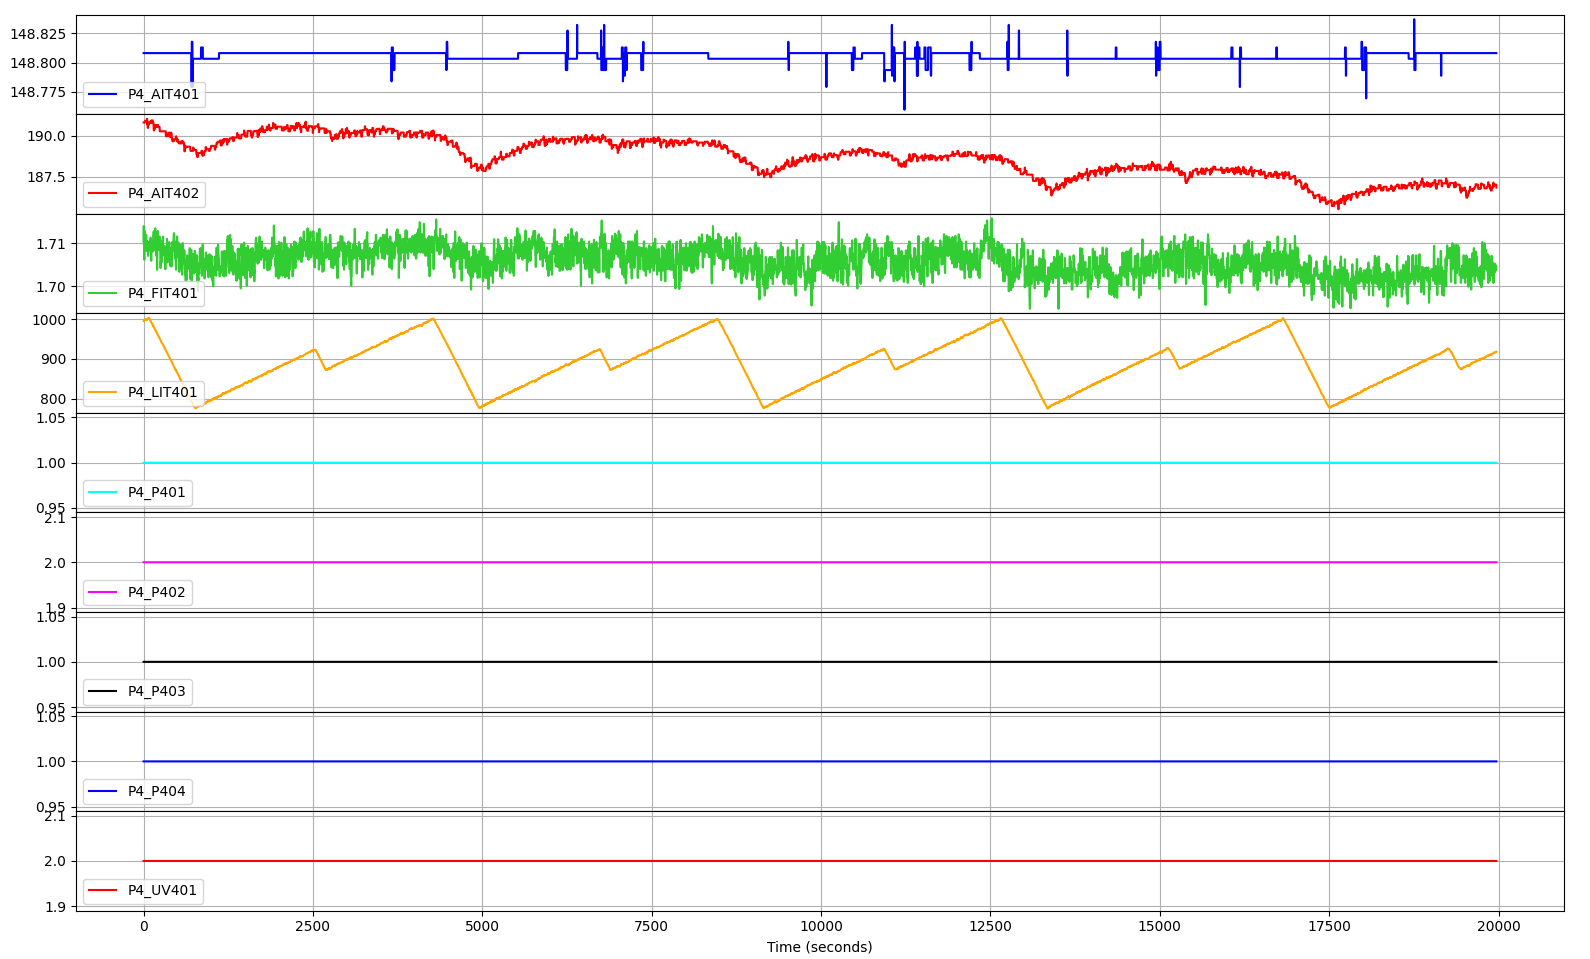
\includegraphics[scale=0.35]{chap6/P4_1.png}
	\caption{PLC4 registers}
	\label{fig:6_graph_P4}
\end{figure}

The image reveals interesting behavior in the \texttt{P4\_AIT401} and \texttt{P4\_AIT401} registers. Notably, \texttt{P4\_AIT401} exhibits a linear trend rather than a cyclic one, with values oscillating within a narrow range. This suggests that, similar to \texttt{P2\_AIT201} (refer to Section \ref{subsubsec:6_P2P3_graphs}), this register may correspond to a sensor measuring a specific water property. On the other hand, \texttt{P4\_AIT402} appears to follow the level trend of sensor \texttt{P4\_LIT401}, but with a downward cyclic pattern where each cycle starts at a lower level than the previous one. Given the limited value range and the similarity in naming conventions, it is highly likely that this register represents another water property sensor rather than a tank.

Additionally, \texttt{P4\_FIT401} does not display a cyclic pattern like the other registers of the same type, and its values exhibit minimal variation, corroborating the findings from the previous analysis phase.

\bigskip
Now, let us refer to Figure \ref{fig:6_graph_P3P4_mv302} to seek confirmation regarding the conjecture that implicates valve \texttt{P3\_MV302} as the responsible actuator for tank filling.

\begin{figure}[ht]
	\centering
	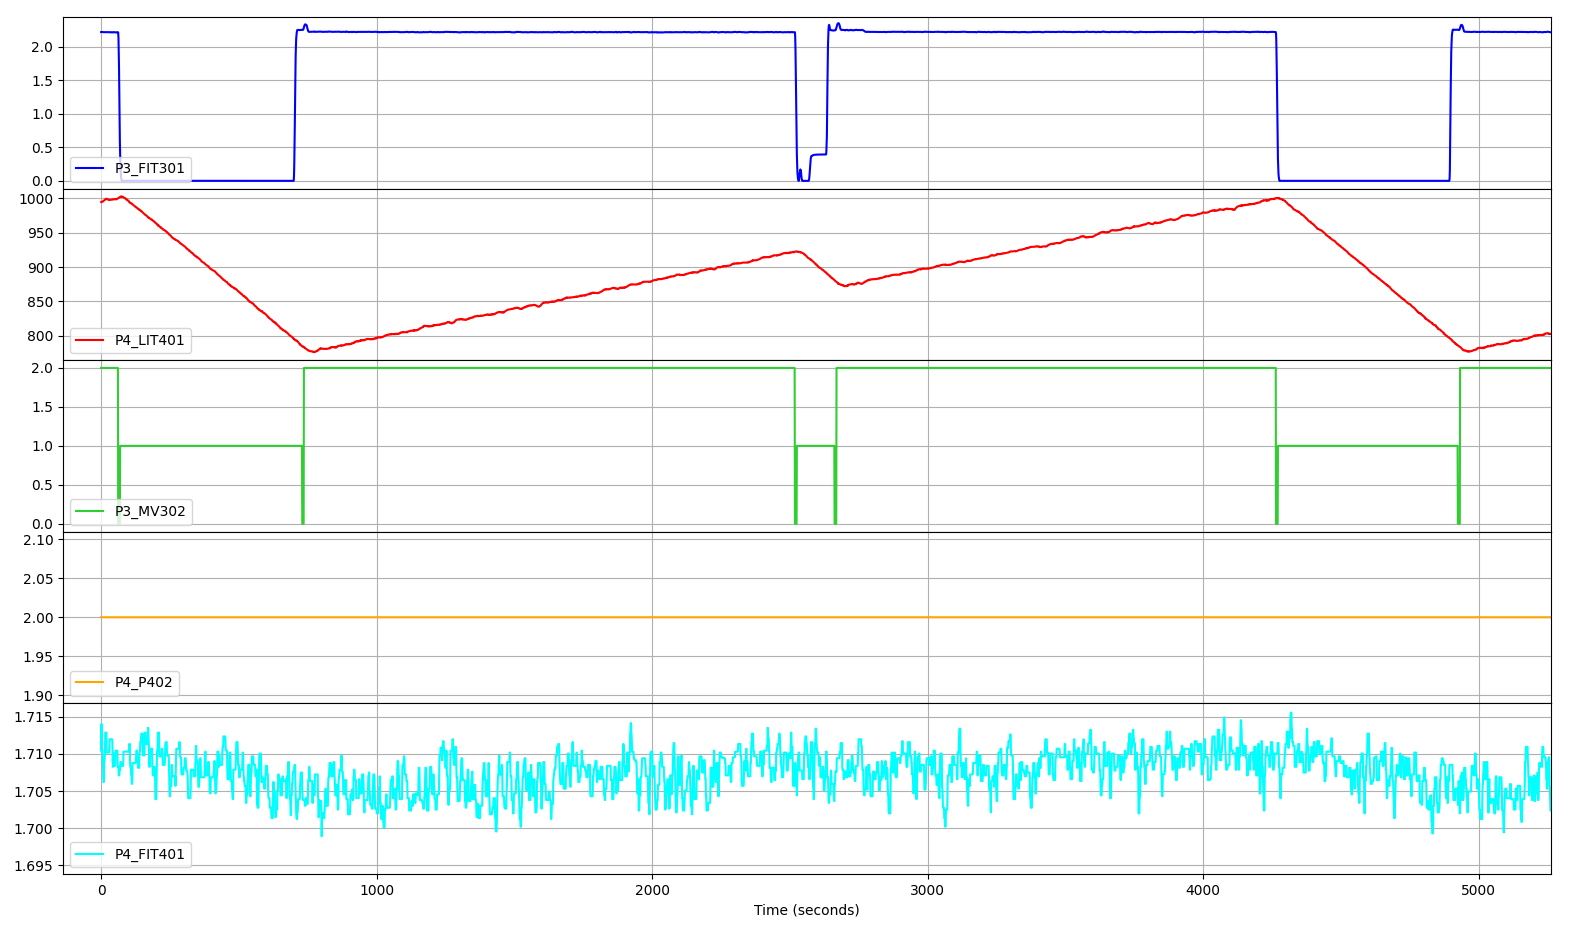
\includegraphics[scale=0.35]{chap6/P3P4_mv302.png}
	\caption{\texttt{P3\_MV302} and \texttt{P4\_LIT401} behaviors}
	\label{fig:6_graph_P3P4_mv302}
\end{figure}

The image provides clear evidence that the behaviors of valve \texttt{P3\_MV302} and tank level sensor \texttt{P4\_LIT401} perfectly align. Additionally, \texttt{P3\_FIT301} (and its corresponding sensor, \texttt{P3\_DPIT301}) appear to be related to the pattern observed in \texttt{P4\_LIT401}.
 
\bigskip
Upon closer observation, it becomes apparent that the tank controlled by PLC4 \textbf{does \textit{not} have plateau periods}. When the incoming water flow ceases, the tank immediately begins to empty. Based on our findings in previous subsystems, we speculate that the actuator responsible for tank emptying could be the pump indicated by register \texttt{P4\_P402}. This speculation is further supported by the nearly constant trend observed in sensor \texttt{P4\_FIT401}.

\bigskip
Figure \ref{fig:6_graph_P3P4_tanks} depicts the correlation between the tanks within this subsystem and the actuators that are responsible for their filling cycle.

\begin{figure}[ht]
	\centering
	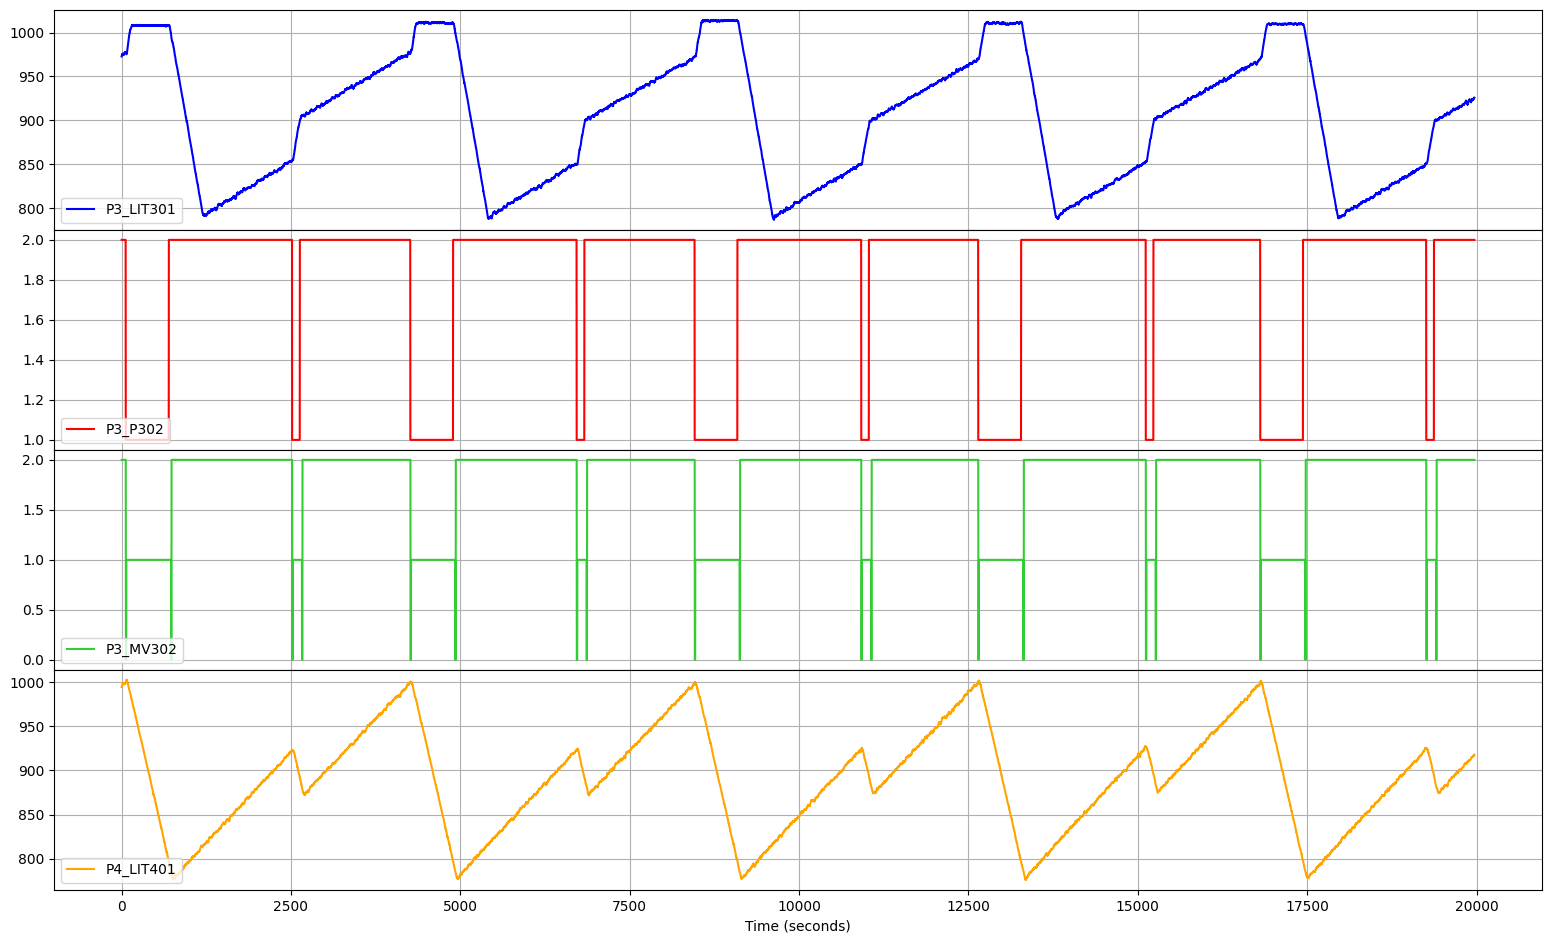
\includegraphics[scale=0.35]{chap6/P3P4_tanks.png}
	\caption{Tanks in subsystem PLC3-4 and their correlation.}
	\label{fig:6_graph_P3P4_tanks}
\end{figure}

\bigskip
Further analysis was conducted to investigate whether valves \texttt{P3\_MV301}, \texttt{P3\_MV303}, and \texttt{P3\_MV304} played a role in the tank filling cycle of PLC4. However, the analysis did not confirm this hypothesis. Therefore, it can be speculated that these valves are connected to other parts of the system that are not currently discussed in this analysis.

\subsubsection{Invariant Inference and Analysis}
\label{subsubsec:6_P3P4_invariants}
The invariant analysis for the subsystem consisting of PLC3-4 will be brief as the states of the subsystem align with the states of valve \texttt{P3\_MV302}, with \texttt{P4\_P402} being constant throughout.

\paragraph{General Invariants}
\label{par:6_P3P4_general_invariant}
Again, the analysis of the general invariants offers no new information compared to what we conjectured earlier. We therefore continue with the analysis of the current system configuration.

\paragraph{Analysis of the Current System Configuration}
\label{par:6_P3P4_current_system_conf}
The analysis of the current system configuration provides confirmation that when the system is in the state \texttt{[P3\_MV302 == 1, P4\_P402 == 2]}, the tank level, as indicated by sensor \texttt{P4\_LIT401}, shows a decreasing slope. Additionally, it is noted that the spare actuators align with the expected behavior. 

However, in the state \texttt{[P3\_MV302 == 2, P4\_P402 == 2]}, the invariants generated by Daikon do not provide the anticipated slope data, which was expected to be increasing based on previous observations. This is due to the descending slope between levels 880 and 925 of the tank represented by \texttt{P4\_LIT401}: by refining the analysis between the two increasing slope sections we get the correct outcome, as shown in Listing \ref{lst:6_preproc_P3P4_refine_analysis}.

\begin{lstlisting}[language=bash, numbers=left, caption=Daikon manual analysis for \texttt{P3\_MV302 == 2}, label=lst:6_preproc_P3P4_refine_analysis]
	===========================
	P3_MV302 == 2 && P4_P402 == 2 && P4_LIT401 < 990 && P4_LIT401 > 930
	===========================
	...
	slope_P4_LIT401 == slope_P3_LIT301 == P4_P404 == P4_P403 == P4_P401 == P3_P301 == P3_MV304 == P3_MV303 == P3_MV301 == 1.0
	...
\end{lstlisting}

\subsubsection{Business Process Mining and Analysis}
\label{subsubsec:6_P3P4_bpa}

The process mining step for the PLC3-4 subsystem is straightforward. In this phase, we will not focus on determining the chronological order of states (as we already know they correspond to the states of valve \texttt{P3\_MV302}). Instead, we will examine the setpoints and extract any available information concerning additional measurements.
Figure \ref{fig:6_P3P4_process_mining} presents the activity diagram depicting the subsystem under analysis.

\begin{figure}[ht]
	\centering
	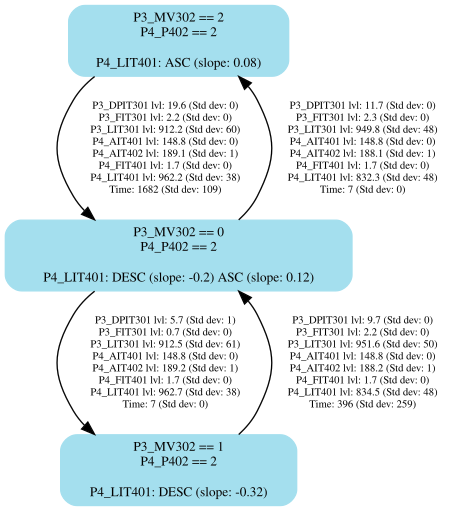
\includegraphics[scale=0.60]{chap6/business_process_P3P4.png}
	\caption{Activity diagram for PLC3-4}
	\label{fig:6_P3P4_process_mining}
\end{figure}

\bigskip
The diagram provides confirmation that when the system is in the state \texttt{[P3\_MV302 == 2, P4\_P402 == 2]}, the tank level trend is increasing. Conversely, when the system is in the state \texttt{[P3\_MV302 == 2, P4\_P402 == 2]}, the trend is decreasing.

\bigskip
Regarding the setpoints, based on the standard deviation of the data from \texttt{P4\_LIT401}, the absolute setpoints for the system are as follows: 785 (minimum), 880 (relative minimum), 925 (relative maximum), and 1000 (maximum).

\bigskip
Furthermore, from the process mining phase, we can extract information about \texttt{P3\_FIT301} and \texttt{P3\_DPIT301}. \texttt{P3\_FIT301} registers values greater than 2 when both pump \texttt{P4\_P402} and valve \texttt{P3\_MV302} are in the ON state, while it drops to an average of 0.7 when the valve is off. Similarly, P3\_DPIT301 registers values close to 20 when the valve is ON, and these values decrease when the valve is OFF.

\subsubsection{Properties}
\label{subsubsec:6_P3P4_summary_table}

Table \ref{table:6_P3P4_summarize_properties} provides a summary of the properties inferred from the conjectures made throughout the different stages of the analysis. Regrettably, we encountered difficulties in determining the type and purpose of the register labeled as \texttt{P4\_UV401}.

\bigskip
{\footnotesize
	\begin{longtable}[l]{p{0.05\textwidth} p{0.57\textwidth} p{0.30\textwidth}}
		\hline
		\textbf{\#} & \textbf{Statement} & \textbf{Derived from} \\
		\hline
		
		P37 & The registers \texttt{P4\_AIT401}, \texttt{P4\_AIT402}, \texttt{P4\_FIT401}, and \texttt{P4\_LIT401} of PLC4 hold likely sensor measurements. & Preliminary Analysis\newline Graphical Analysis \\
		\hline
		
		P38 & The register \texttt{P4\_P402} of PLC4 holds likely actuator command. Its status is constantly ON. & Preliminary Analysis\newline Graphical Analysis\newline Business Process \\
		\hline
		
		P39 & The registers \texttt{P4\_P401}, \texttt{P4\_P403}, and \texttt{P4\_P404} of PLC4 are associated to spare actuators. & Preliminary Analysis\newline Graphical Analysis\newline Invariant Analysis \\
		\hline
		
		P40 & The register \texttt{P4\_LIT401} of PLC4 is associated to the level sensor of the tank controlled by PLC4. & Preliminary Analysis\newline Graphical Analysis \\
		\hline
		
		P41 & \texttt{P3\_MV302} and \texttt{P4\_P402} are the actuators responsible for the level behavour of the water contanined in the tank controlled by PLC4. & Graphical Analysis\newline Invariant Analysis\newline Business Process \\
		\hline
		
		P42 & The level of the tank identified by the register \texttt{P4\_LIT401} increases when both \texttt{P3\_MV302} and \texttt{P4\_P402} are in the ON state. It decreases when \texttt{P3\_MV302} is in the OFF state. & Graphical Analysis\newline Invariant Analysis\newline Business Process \\
		\hline
		
		P43 & The trend of the tank level controlled by PLC4 transition from ascending to descending when the level reaches approximately 925 and 1000. It changes from descending when the level reaches approximately 785 and 880. & Business Process \\
		\hline
		
		P44 & Absolute setpoints are 785, 880, 925 and 1000 & Business Process \\
		\hline
		
		P45 & \texttt{P4\_FIT401} serves as a flow or pressure sensor to the \texttt{P4\_LIT401} register. It is related to the \texttt{P4\_P402} pump. & Graphical Analysis\newline Business Process \\
		\hline
		
		P46 & \texttt{P4\_P401} does not exhibit a cyclic trend. & Graphical Analysis \\
		\hline
		
		P47 & The register \texttt{P4\_P402} exhibits a cyclic decreasing trend, which is closely linked to the trend observed in the \texttt{P4\_LIT401} register. & Graphical Analysis\\
		\hline
		
		P48 & Both \texttt{P4\_AIT401} and \texttt{P4\_AIT402} serves as sensors for measuring certain properties of the water. & Preliminary Analysis\newline Graphical Analysis \\
		\hline
		
		P49 & The registers \texttt{P3\_MV301}, \texttt{P3\_MV303}, and \texttt{P3\_MV304} do not have an impact on the water level dynamics on the tank controlled by PLC4. & Graphical Analysis\newline Business Process \\
		\hline
		
		\caption{Properties of the PLC3-4 subsystem}
		\label{table:6_P3P4_summarize_properties}
	\end{longtable}
}

\section{PLCs Architecture}
In Table \ref{table:6_plc_registers_summary}, we present an overview of the architecture of the four analyzed PLCs derived from the previous phases of the analysis. For each PLC, we provide details about its constituent registers, including their operational range. Where possible, we also indicate the role of these registers within the physical system. By combining the information presented in Tables \ref{table:6_P1P2_summarize_properties}, \ref{table:6_P2P3_summarize_properties}, and \ref{table:6_P3P4_summarize_properties} with the content of Table \ref{table:6_plc_registers_summary}, we can consider the reverse engineering process implemented in this analysis to be complete. 
To enhance readability, we will assign integer numbers to tanks based on the PLCs that control them. For example, Tank 1 represents the tank associated with PLC1, Tank 3 represents the tank associated with PLC3, and so forth.

\bigskip
{\small
	\begin{longtable}[c]{p{0.10\textwidth} p{0.50\textwidth} p{0.13\textwidth} p{0.18\textwidth}}
		\hline
		\textbf{PLC} & \textbf{Physical device / Variable} & \textbf{Range} & \textbf{PLC register} \\ [0.5ex] 
		\hline
		\multirow{5}{12em}{PLC1} & Level sensor for Tank 1 & [489-815] & \texttt{P1\_LIT101} \\ 
		& Flow or pressure sensor & [0-2.7] & \texttt{P1\_FIT101} \\
		& Valve for Tank 1 inflow water & \{0,1,2\} & \texttt{P1\_MV101} \\ 
		& Pump for Tank 1 outflow water & \{0,1\} & \texttt{P1\_P101} \\
		& Spare actuator (OFF) & 1 & \texttt{P1\_P102} \\
		\hline
		\multirow{11}{12em}{PLC2} & Flow or pressure sensor & [0-2.4] & \texttt{P2\_FIT201} \\
		& Sensor for some water property & [252-256] & \texttt{P2\_AIT201} \\
		& Sensor for some water property & [8.3-8.4] & \texttt{P2\_AIT202} \\
		& Unkown & [320-342] & \texttt{P2\_AIT203} \\
		& Valve for Tank 3 inflow water & \{0,1,2\} & \texttt{P2\_MV201} \\
		& Spare actuator (OFF) & 1 & \texttt{P2\_P201} \\
		& Spare actuator (OFF) & 1 & \texttt{P2\_P202} \\
		& Pump (unknown role) & \{0.1\} & \texttt{P2\_P203} \\
		& Spare actuator (OFF) & 1 & \texttt{P2\_P204} \\
		& Pump (unknown role) & \{0.1\} & \texttt{P2\_P205} \\
		& Spare actuator (OFF) & 1 & \texttt{P2\_P206} \\
		\hline
		\multirow{9}{12em}{PLC3} & Level sensor for Tank 3 & [768-1014] & \texttt{P3\_LIT301} \\
		& Flow or pressure sensor & [0-2.4] & \texttt{P3\_FIT301} \\
		& Flow or pressure sensor & [0-20.4] & \texttt{P3\_DPIT301} \\
		& Valve (unkonw role) & \{0,1,2\} & \texttt{P3\_MV301} \\
		& Valve for Tank 4 inflow water & \{0,1,2\} & \texttt{P3\_MV302} \\
		& Valve (unkonw role) & \{0,1,2\} & \texttt{P3\_MV303} \\
		& Valve (unkonw role) & \{0,1,2\} & \texttt{P3\_MV304} \\
		& Spare actuator (OFF) & 1 & \texttt{P3\_P301} \\
		& Pump for Tank 3 outflow water & [0,1] & \texttt{P3\_P302} \\
		\hline
		\multirow{9}{12em}{PLC4} & Level sensor for Tank 4 & [775-1002] & \texttt{P4\_LIT401} \\
		& Flow or pressure sensor & [1.7] & \texttt{P4\_FIT401} \\
		& Sensor for some water property & [148.8] & \texttt{P4\_AIT401} \\
		& Sensor for some water property & [185-191] & \texttt{P4\_AIT402} \\
		& Spare actuator & 1 & \texttt{P4\_P401} \\
		& Pump for Tank 4 outflow water & 2 & \texttt{P4\_P402} \\
		& Spare actuator & 1 & \texttt{P4\_P403} \\
		& Spare actuator & 1 & \texttt{P4\_P404} \\
		& Unknown & 2 & \texttt{P4\_UV401} \\
		\hline
		
		\caption{Summary of the reconstructed composition PLCs from 1 to 4 in the iTrust SWaT System}
		\label{table:6_plc_registers_summary}
	\end{longtable}
}
\vfill
%\nolinenumbers